\documentclass[12pt,a4paper]{report}

\usepackage{styles/dolgozat}

\usepackage{listings}
\usepackage{styles/cpp}
\usepackage{styles/python}

\usepackage{hyperref}


\usepackage{tabularx}
\newcolumntype{Y}{>{\centering\arraybackslash}X}
\usepackage{hhline}

\usepackage{placeins}
\usepackage{float}


\begin{document}

\pagestyle{empty} %a címlapon ne legyen semmi=empty, azaz nincs fejléc és lábléc

% A Miskolci Egyetem címere
{\large
\begin{center}
\vglue 1truecm
\textbf{\huge\textsc{Szakdolgozat}}\\
\vglue 1truecm

\includegraphics[width=4.8truecm, height=4truecm]{images/me_logo.png}\\
\textbf{\textsc{Miskolci Egyetem}}
\end{center}}

\vglue 1.5truecm %függõleges helykihagyás

% A szakdolgozat címe, akár több sorban is
{\LARGE
\begin{center}
\textbf{Webalkalmazások adatainak perzisztens tárolása gráfadatbázisok segítségével}
\end{center}}

\vspace*{2.5truecm}
% A hallgató neve, évfolyam, szak(ok), a konzulens(ek) neve
{\large
\begin{center}
\begin{tabular}{c}
\textbf{Készítette:}\\
Kévés Levente\\
Programtervező informatikus
\end{tabular}
\end{center}
\begin{center}
\begin{tabular}{c}
\textbf{Témavezető:}\\
Piller Imre
\end{tabular}
\end{center}}
\vfill
% Keltezés: Hely, év
{\large
\begin{center}
\textbf{\textsc{Miskolc, 2022}}
\end{center}}

\newpage


\newpage

\pagestyle{empty}

%Feladatkiiras
\begin{flushleft}
\textsc{\bfseries Miskolci Egyetem}\\
Gépészmérnöki és Informatikai Kar\\
Alkalmazott Matematikai Intézeti Tanszék\hspace*{4cm}\hfil \textbf{Szám:}
\end{flushleft}
\vskip 0.5cm
\begin{center}
\large\textsc{\bfseries Szakdolgozat Feladat}
\end{center}
\vskip 0.5cm
Kévés Levente (IG9GGV) Programtervező informatikus jelölt részére.\newline

\noindent\textbf{A szakdolgozat tárgyköre:} Gráfadatbázisok\newline

\noindent\textbf{A szakdolgozat címe:} \\
Webalkalmazások adatainak perzisztens tárolása gráfadatbázisok segítségével\newline

\noindent\textbf{A feladat részletezése:}

\medskip

\emph{Webalkalmazások fejlesztése kapcsán jellemzően igény van az adatok perzisztens tárolására. A hagyományosnak tekinthető megközelítést a relációs adatmodellt alkalmazó, tipikusan SQL lekérdezőnyelvű relációs adatbázisrendszerek adják. Ezek mellett egyre nagyobb népszerűségre tesznek szert például a NoSQL adatbázisok. A dolgozat egy könyvtári nyilvántartás példáján keresztül vizsgálja meg, hogy milyen adatmodellek állnak rendelkezésre, majd ezek közül a gráfadatbázisok témájával foglalkozik részletesebben. A Neo4j adatbázismotort és a Cypher lekérdezőnyelvet felhasználva mutatja meg, hogy milyen előnyei és hátrányai vannak az adatok ilyen módú kezelésének egy webalkalmazás esetében. Az alkalmazás többségében JavaScript nyelven készül. A frontend a React keretrendszer, a backend pedig NodeJS segítségével valósul meg.}

\vfill

\noindent\textbf{Témavezető:} Piller Imre (egyetemi tanársegéd) \newline

% \noindent\textbf{Konzulens(ek):} (akkor kötelezõ, ha a témavezetõ nem valamelyik matematikai tanszékrõl való; de persze lehet egyébként is)\newline

\noindent\textbf{A feladat kiadásának ideje:} 2021. szeptember 27.\newline

%\noindent\textbf{A feladat beadásának határideje:}

\vskip 2cm

\hbox to \hsize{\hfil{\hbox to 6cm {\dotfill}\hbox to 1cm{}}}

\hbox to \hsize{\hfil\hbox to 3cm {szakfelelős}\hbox to 2cm{}}

\newpage

\vspace*{1cm}  
\begin{center}
\large\textsc{\bfseries Eredetiségi Nyilatkozat}
\end{center}
\vspace*{2cm}  

Alulírott \textbf{Kévés Levente}; Neptun-kód: \texttt{IG9GGV} a Miskolci Egyetem Gépészmérnöki és Informatikai Karának végzős Programtervező informatikus szakos hallgatója ezennel büntetőjogi és fegyelmi felelősségem tudatában nyilatkozom és aláírásommal igazolom, hogy \textit{Webalkalmazások adatainak perzisztens tárolása gráfadatbázisok segítségével}
című szakdolgozatom saját, önálló munkám; az abban hivatkozott szakirodalom
felhasználása a forráskezelés szabályai szerint történt.\\

Tudomásul veszem, hogy szakdolgozat esetén plágiumnak számít:
\begin{itemize}
\item szószerinti idézet közlése idézőjel és hivatkozás megjelölése nélkül;
\item tartalmi idézet hivatkozás megjelölése nélkül;
\item más publikált gondolatainak saját gondolatként való feltüntetése.
\end{itemize}

Alulírott kijelentem, hogy a plágium fogalmát megismertem, és tudomásul veszem, hogy
plágium esetén szakdolgozatom visszautasításra kerül.

\vspace*{3cm}

\noindent Miskolc, \hbox to 2cm{\dotfill} .év \hbox to 2cm{\dotfill} .hó \hbox to 2cm{\dotfill} .nap

\vspace*{3cm}

\hspace*{8cm}\begin{tabular}{c}
\hbox to 6cm{\dotfill}\\
Hallgató
\end{tabular}



\newpage

\noindent 1.

\begin{tabular}{cl}
&szükséges (módosítás külön lapon) \\
A szakdolgozat feladat módosítása& \\
& nem szükséges\\
&\\
\hbox to 4cm{\dotfill}&\multicolumn{1}{c}{\hbox to 5cm{\dotfill}}\\
dátum& \multicolumn{1}{c}{témavezető(k)}
\end{tabular}
\vskip1.5mm

\noindent 2. A feladat kidolgozását ellenőriztem:

\vskip1.5mm

\begin{tabular}{l@{\hspace*{4cm}}l}
témavezető (dátum, aláírás):& konzulens (dátum, aláírás):\\
\dotfill&\dotfill\\
\dotfill&\dotfill\\
\dotfill&\dotfill
\end{tabular}

\vskip1.5mm

\noindent 3. A szakdolgozat beadható:

\vskip1.5mm

\begin{tabular}{@{\hspace*{1.3cm}}c@{\hspace*{2.1cm}}c}
\hbox to 4cm{\dotfill}&\multicolumn{1}{c}{\hbox to 5cm{\dotfill}}\\
dátum& \multicolumn{1}{c}{témavezető(k)}
\end{tabular}

\vskip1.5mm

\noindent 4.
\begin{tabular}[t]{@{}l@{\hspace*{1mm}}l@{\hspace*{1mm}}l@{}}
A szakdolgozat& \hbox to 3.5cm{\dotfill} &szövegoldalt\\
              & \hbox to 3.5cm{\dotfill} &program protokollt (listát, felhasználói leírást)\\
              &\hbox to 3.5cm{\dotfill}   &elektronikus adathordozót (részletezve)\\
              &\hbox to 3.5cm{\dotfill} & \\
              &\hbox to 3.5cm{\dotfill} &egyéb mellékletet (részletezve)\\
              &\hbox to 3.5cm{\dotfill} &\\
\end{tabular}
\newline tartalmaz.

\vskip1.5mm

\begin{tabular}{@{\hspace*{1.3cm}}c@{\hspace*{2.1cm}}c}
\hbox to 4cm{\dotfill}&\multicolumn{1}{c}{\hbox to 5cm{\dotfill}}\\
dátum& \multicolumn{1}{c}{témavezető(k)}
\end{tabular}

\noindent 5.

\begin{tabular}{ll}
&bocsátható\\
A szakdolgozat bírálatra& \\
& nem bocsátható\\
\end{tabular}

\vskip1.5mm

\noindent A bíráló neve: \hbox to 8cm{\dotfill}

\vskip4mm

\begin{tabular}{@{\hspace*{1.3cm}}c@{\hspace*{2.1cm}}c}
\hbox to 4cm{\dotfill}&\multicolumn{1}{c}{\hbox to 5cm{\dotfill}}\\
dátum& \multicolumn{1}{c}{szakfelelős}
\end{tabular}

\noindent 6.
\begin{tabular}[t]{@{}l@{\hspace*{1mm}}l@{\hspace*{1mm}}l@{}}
A szakdolgozat osztályzata& &\\
&a témavezető javaslata:& \hbox to 3cm{\dotfill}\\
&a bíráló javaslata:& \hbox to 3cm{\dotfill}\\
&a szakdolgozat végleges eredménye:& \hbox to 3cm{\dotfill}
\end{tabular}

\vspace*{4mm}

\noindent Miskolc, \hbox to 4.5cm{\dotfill} \hspace*{2.5cm}
\begin{tabular}[t]{cc}
\hbox to 6cm{\dotfill}\\
a Záróvizsga Bizottság Elnöke
\end{tabular}


\cleardoublepage
\pagenumbering{gobble}
\tableofcontents
\cleardoublepage
\pagenumbering{arabic}

\newpage

\pagestyle{fancy}

\Chapter{Bevezetés}

% Ezt elegendő csak a végén összerakni, amikor már lehet látni egyben, hogy pontosan mi és hogy készült el (nem csak program, de dolgozat szintjén is).

% TODO: Itt a gráfadatbázisokról kellene úgy általában egy rövid (esetleg akár kissé promóció jellegű) leírásnak lennie.

% TODO: Röviden említeni kellene, hogy könyvtáras példáról lesz szó. Indokolni kellene, hogy a könyvtáras példa miért tünt megfelelőnek.

% TODO: Fel kellene sorolni, hogy milyen összehasonlításokra, és vizsgálatokra kerül majd sor.

A dolgozat négy nagyobb fejezetből áll. Ezek közül az első a Gráfadatbázisok című fejezet.
Ebben a fejezetben először a különböző adatbázis paradigmák kerülnek bemutatásra. Ezt követően az adatok gráfokkal való leírásáról lesz szó, majd néhány elterjedt gráfadatbázis kerül bemutatásra

\bigskip

A minta alkalmazás fejezet során az elkészült alkalmazás kerül részletes bemutatásra. Először az alkalmazás szerepkörei, illetve használati esetei kerülnek bemutatásra. Ezt követően az alkalmazás funkcióiról lesz szó, azaz hogy egy felhasználó mi mindent tud csinálni az alkalmazáson belül. Ez után az alkalmazás architektúrájának ismeretesére és az API bemutatására fog sor kerülni. Ezt követi majd az alkalmazás és a backend megvalósításának leírása.

\bigskip

Ezt követi a Neo4j gráfadatbázist bemutató fejezet. Először a Neo4j által nyújtott szolgáltatások lesznek ismertetve, majd egy rövid leírás arról, hogy hogyan lehet adatokat tárolni a Neo4j féle gráfadatbázisban. Ezt után a Neo4j által használt Cypher lekérdező nyelv kerül összehasonlításra az SQL-el. A fejezet az alkalmazás és az adatbázis összekapcsolásának menetéről, valamint a magasabb szintű hozzáférési módok ismertetéséről fog szólni.

\bigskip

Az utolsó nagyobb fejezet Optimalizálás és adatbázis menedzsment névre hallgat. Ebben a fejezeten webalkalmazások és adatbázisok jogosultságkezelése és gyorsítótárazása lesz röviden ismertetve, majd a Neo4j gráfadatbázis kongifurálási lehetőségei kerülnek bemutatásra. Végül pedig a Neo4j által biztosított biztonsági mentési lehetőségek lesznek bemutatva.
\Chapter{Gráfadatbázisok}

% TODO: Itt amit csak lehet hivatkozni kellene. A dolgozatban lévő hivatkozások jelentős része kerülhet ebbe a fejezetbe.
Ebben a fejezetben szó lesz arról, hogy milyen adatbázis paradigmák vannak, hogyan lehet adatokat gráfokkal leírni,  valamint hogy milyen elterjedt gráfadatbázisok vannak.

\Section{Paradigmák}

% TODO: Itt ki kellene fejteni, hogy milyen jellemző adatbázis paradigmák vannak. (Múltkor a 4 fő típust említettem, de Lehet itt 7 is.)

% https://tudip.com/blog-post/7-database-paradigms/

% https://arato.inf.unideb.hu/ispany.marton/Database/Lectures2020/noSQL.pdf
% http://eta.bibl.u-szeged.hu/5031/7/EFOP343_A6_7e_BigData-nosql-over-hadoop-SPOC.pdf
% https://inf.mit.bme.hu/sites/default/files/publications/nosql-konyvfejezet.pdf
Ebben az alfejezetben 7 adatbázis paradigma kerül bemutatásra. \cite{paradigms} \cite{nosql1} \cite{nosql2} \cite{nosql3}

\subsection{Kulcs-érték adatbázis}

Ez az adatbázis típus kulcs-érték párokban tárolja az adatokat.  Az adatokat a kulcsok segítségével gyorsan el lehet érni, viszont ezen kívül jellemzően nem lehet másfajta lekérdezéseket végrehajtani. Ilyen adatbázisok például a Redis, a Memcached és a Riak.

\subsection{Oszlopalapú adatbázis}
Szokás még oszlopcsalád adatbázisnak, vagy oszlop adatbázisnak is nevezni. Az oszlopalapú adatbázis hasonlít a kulcs-érték adatbázishoz, ugyanis itt is kulcs-érték páronként vannak tárolva az adatok, de az érték oszlopokban kerülnek tárolásra. Egy oszlophoz jellemzően tartozik egy kulcs, egy érték, és egy időbélyeg. Nincs hozzá séma, ezért csak szervezetlen adatok tárolására alkalmas. A CQL (Cassandra Query Language) segítségével lehet lekérdezéseket írni, viszont nincsenek join műveletek. Ilyen adatbázisok például a Cassandra, az HBase és a BigTable.

\subsection{Dokumentum adatbázis}
A dokumentum adatbázis dokumentumok tárolására és lekérésére szolgálnak. A dokumentumok önleíróak, hierarchikus szerkezetűek, kollekciókat és skalár értékeket tartalmazhatnak. A dokumentumok lehetnek például JSON, XML vagy YAML formátumokban. Ilyen adatbázisok például a MongoDB, a CouchDB és a Firestore.

\subsection{Relációs adatbázis}
% Bővebben?
A relációs adatbázis a relációs adatmodellen alapszik. Ilyen adatbázisok például az Oracle Database, a MySQL és a Microsoft SQL Server.

\subsection{Gráf adatbázis}
A gráf adatbázis gráfok hatékony tárolására és azokon végzett műveletek gyors végrehajtására ad lehetőséget. Az adatokat csomópontok és élek formájában tárolja. Lehetőséget biztosít komplex lekérdezésekre. Ilyen adatbázisok például a Neo4j, az Amazon Neptune és az Azure Cosmos DB.

\subsection{Teljes szövegű kereső motor}
Teljes szövegű kereső motorra épülő adatbázisban a dokumentumok tartalmát indexelik. Az adatbázisban való kereséskor a keresés az indexen keresztül fog zajlani. Ilyen keresőmotorok például az Apache Lucene és az Elasticsearch

\subsection{Több modelles adatbázis}
Több modelles adatbázis lehetőséget biztosít több fajta adatmodell együttes használatára. Ilyen adatbázisok például a Fauna és az ArangoDB.

% https://neo4j.com/docs/getting-started/current/graphdb-concepts/#graphdb-concepts
\Section{Adatok leírása gráfokkal}
% TODO: Ki kellene térni arra, hogy milyen alternatívák vannak az adattárolásra. Például, hogy
% - Mi kerülhet a csomópontba és az élekbe. (Tehát, hogy melyik változatnál éppen hol van az adata.)
% - Ki kellene térni a típusosság problémakörére.

Gráfadatbázisok esetében az adatok csomópontok, és az azokat összekötő kapcsolatok formájában kerülnek tárolásra. \cite{adatok-leirasa} A csomópontokhoz és a kapcsolatokhoz tartozhatnak tulajdonságok is. Ezek kulcs-érték párok, amik az adott csomóponthoz vagy kapcsolathoz tartozó további információkat tárolnak. A csomópontokat el lehet látni címkékkel is, amik csoportosítják a csomópontokat. Általában a csomópont egy főnév, a kapcsolat egy ige.

\bigskip

Egy csomópont tulajdonságát bizonyos esetekben célszerű lehet külön csomópontként reprezentálni. Például egy gépjárműveket tartalmazó adatbázisban a gépjárművek márkáját lehetne tárolni tulajdonságként a gépjármű csomópontban, de célszerű lehet egy külön csomópontot létrehozni a márkának, köztük egy kapcsolattal.

\Section{Elterjedt gráfadatbázisok}

% TODO: Itt kellene összegyűjteni 6-8 elterjedt, vagy valamilyen szempontból jelentős gráfadatbázist.
Számos elérhető gráfadatbázis szolgáltatás létezik. Ebben az alfejezetben röviden bemutatásra kerül közülük néhány.

% https://neo4j.com/docs/getting-started/current/
\subsection{Neo4j}
A Neo4j a Neo4j, Inc. által fejlesztett gráfadatbázis. \cite{neo4j} Az architektúrát úgy tervezték, hogy az optimális legyen a csomópontok és a kapcsolatok kezelésére, tárolására és bejárására. Tulajdonsággráf megközelítést alkalmaz, ami előnyös bejárási teljesítmény és műveleti futásidő szempontjából. A Cypher lekérdező nyelvet használja, ami SQL jellegű.

% https://docs.aws.amazon.com/neptune/latest/userguide/intro.html
\subsection{Amazon Neptune}
Az Amazon Neptune az Amazon.com, Inc. által fejlesztett gráfadatbázis. \cite{neptune} A Neptune egy gyors, megbízható és teljesen felügyelt gráfadatbázis, amely megkönnyíti a szorosan összekapcsolt adatkészletekkel működő alkalmazások létrehozását és futtatását. A Neptune magja egy erre a célra épített, nagy teljesítményű gráf adatbázis motor. Ez a motor több milliárd kapcsolatok tárolására és a grafikon ezredmásodperces késleltetéssel történő lekérdezésére van optimalizálva. A Neptune támogatja az Apache TinkerPop Gremlin és a W3C SPARQL gráflekérdező nyelveit.

% https://docs.microsoft.com/en-us/azure/cosmos-db/introduction
\subsection{Azure Cosmos DB}
Az Azure Cosmos DB a Microsoft Corporation által fejlesztett gráfadatbázis. \cite{azure} Nagyon gyors válaszidővel, és automatikus és azonnali skálázhatósággal van felszerelve. 99,99\%-os SLA-t (Service-level agreement/Szolgáltatási Szint Megállapodás) kínál. Használható hozzá az Apache TinkerPop Gremlin lekérdező nyelv. 

% https://docs.tigergraph.com/tigergraph-server/current/intro/
\subsection{Tigergraph}
A TigerGraph a TigerGraph által fejlesztett gráfadatbázis. \cite{tigergraph} A TigerGraph biztosít gyors adatbetöltési sebességet grafikonok készítéséhez, párhuzamos gráf-algoritmusok gyors végrehajtását, valós idejű frissítéseket és beillesztéseket a REST segítségével, valamint képes a valós idejű elemzések egyesítésére nagyszabású offline adatfeldolgozással. A GSQL szoftvert használja az adatbázis menedzselésére.

% https://cambridgesemantics.com/anzograph/
% https://docs.cambridgesemantics.com/anzograph/v2.5/userdoc/features.htm
\subsection{AnzoGraph DB}
AnzoGraph DB a Cambridge Semantics által fejlesztett gráfadatbázis. Az AnzoGraph egy natív, masszívan párhuzamos feldolgozású gráf  OLAP (Online Analytics Processing) adatbázis. \cite{anzograph1} \cite{anzograph2} Az adatok natív gráf formátumban kerülnek tárolásra a lemezen vagy a memóriában. A gráf  OLAP technológia lehetővé teszi a felhasználók számára a grafikonok adatainak interaktív megtekintését, elemzését és frissítését. Használhatóak hozzá a SPARQL és a Cypher lekérdező nyelvek.

% https://dgraph.io/docs/dgraph-overview/
\subsection{Dgraph}
A Dgraph a Dgraph Labs által fejlesztett gráfadatbázis. \cite{dgraph} A Dgraph egy horizontálisan méretezhető é GraphQL. A Dgraph a modern alkalmazások és webhelyek működéséhez szükséges nagy tranzakciós terhelésre készült. A GraphQL lekérdező nyelvre épülő DQL-t (Dgraph Query Language) használja.
\Chapter{A minta alkalmazás}

% TODO: Egy rövid áttekintés a könyvtári kölcsönzéses és hasonló célú alkalmazásokról. Jó, hogy ha van néhány hivatkozás is hozzá.

A mintaalkalmazás egy könyvtár adatainak kezelését valósítja meg online felületen. Könyvek böngészésén és kölcsönzésén kívül lehetősége van a felhasználónak könyveket értékelni, hozzászólásokat írni, listákat létrehozni, könyvjelzőket kezelni, valamint új könyvekre igényt leadni. Ebben a fejezetben az alkalmazás által nyújtott funkciók részletes bemutatásáról, valamint azok megvalósításáról lesz szó.

\Section{Szerepkörök, használati esetek}

% TODO: Ide egy felsorolás (esetleg egy use-case diagram) kerülhet az admin és a publikus funkciókról.

Az alkalmazás használati eset (\textit{use-case}) diagramja \aref{fig:use-case}. ábrán található.

\begin{figure}[h]
	\centering
	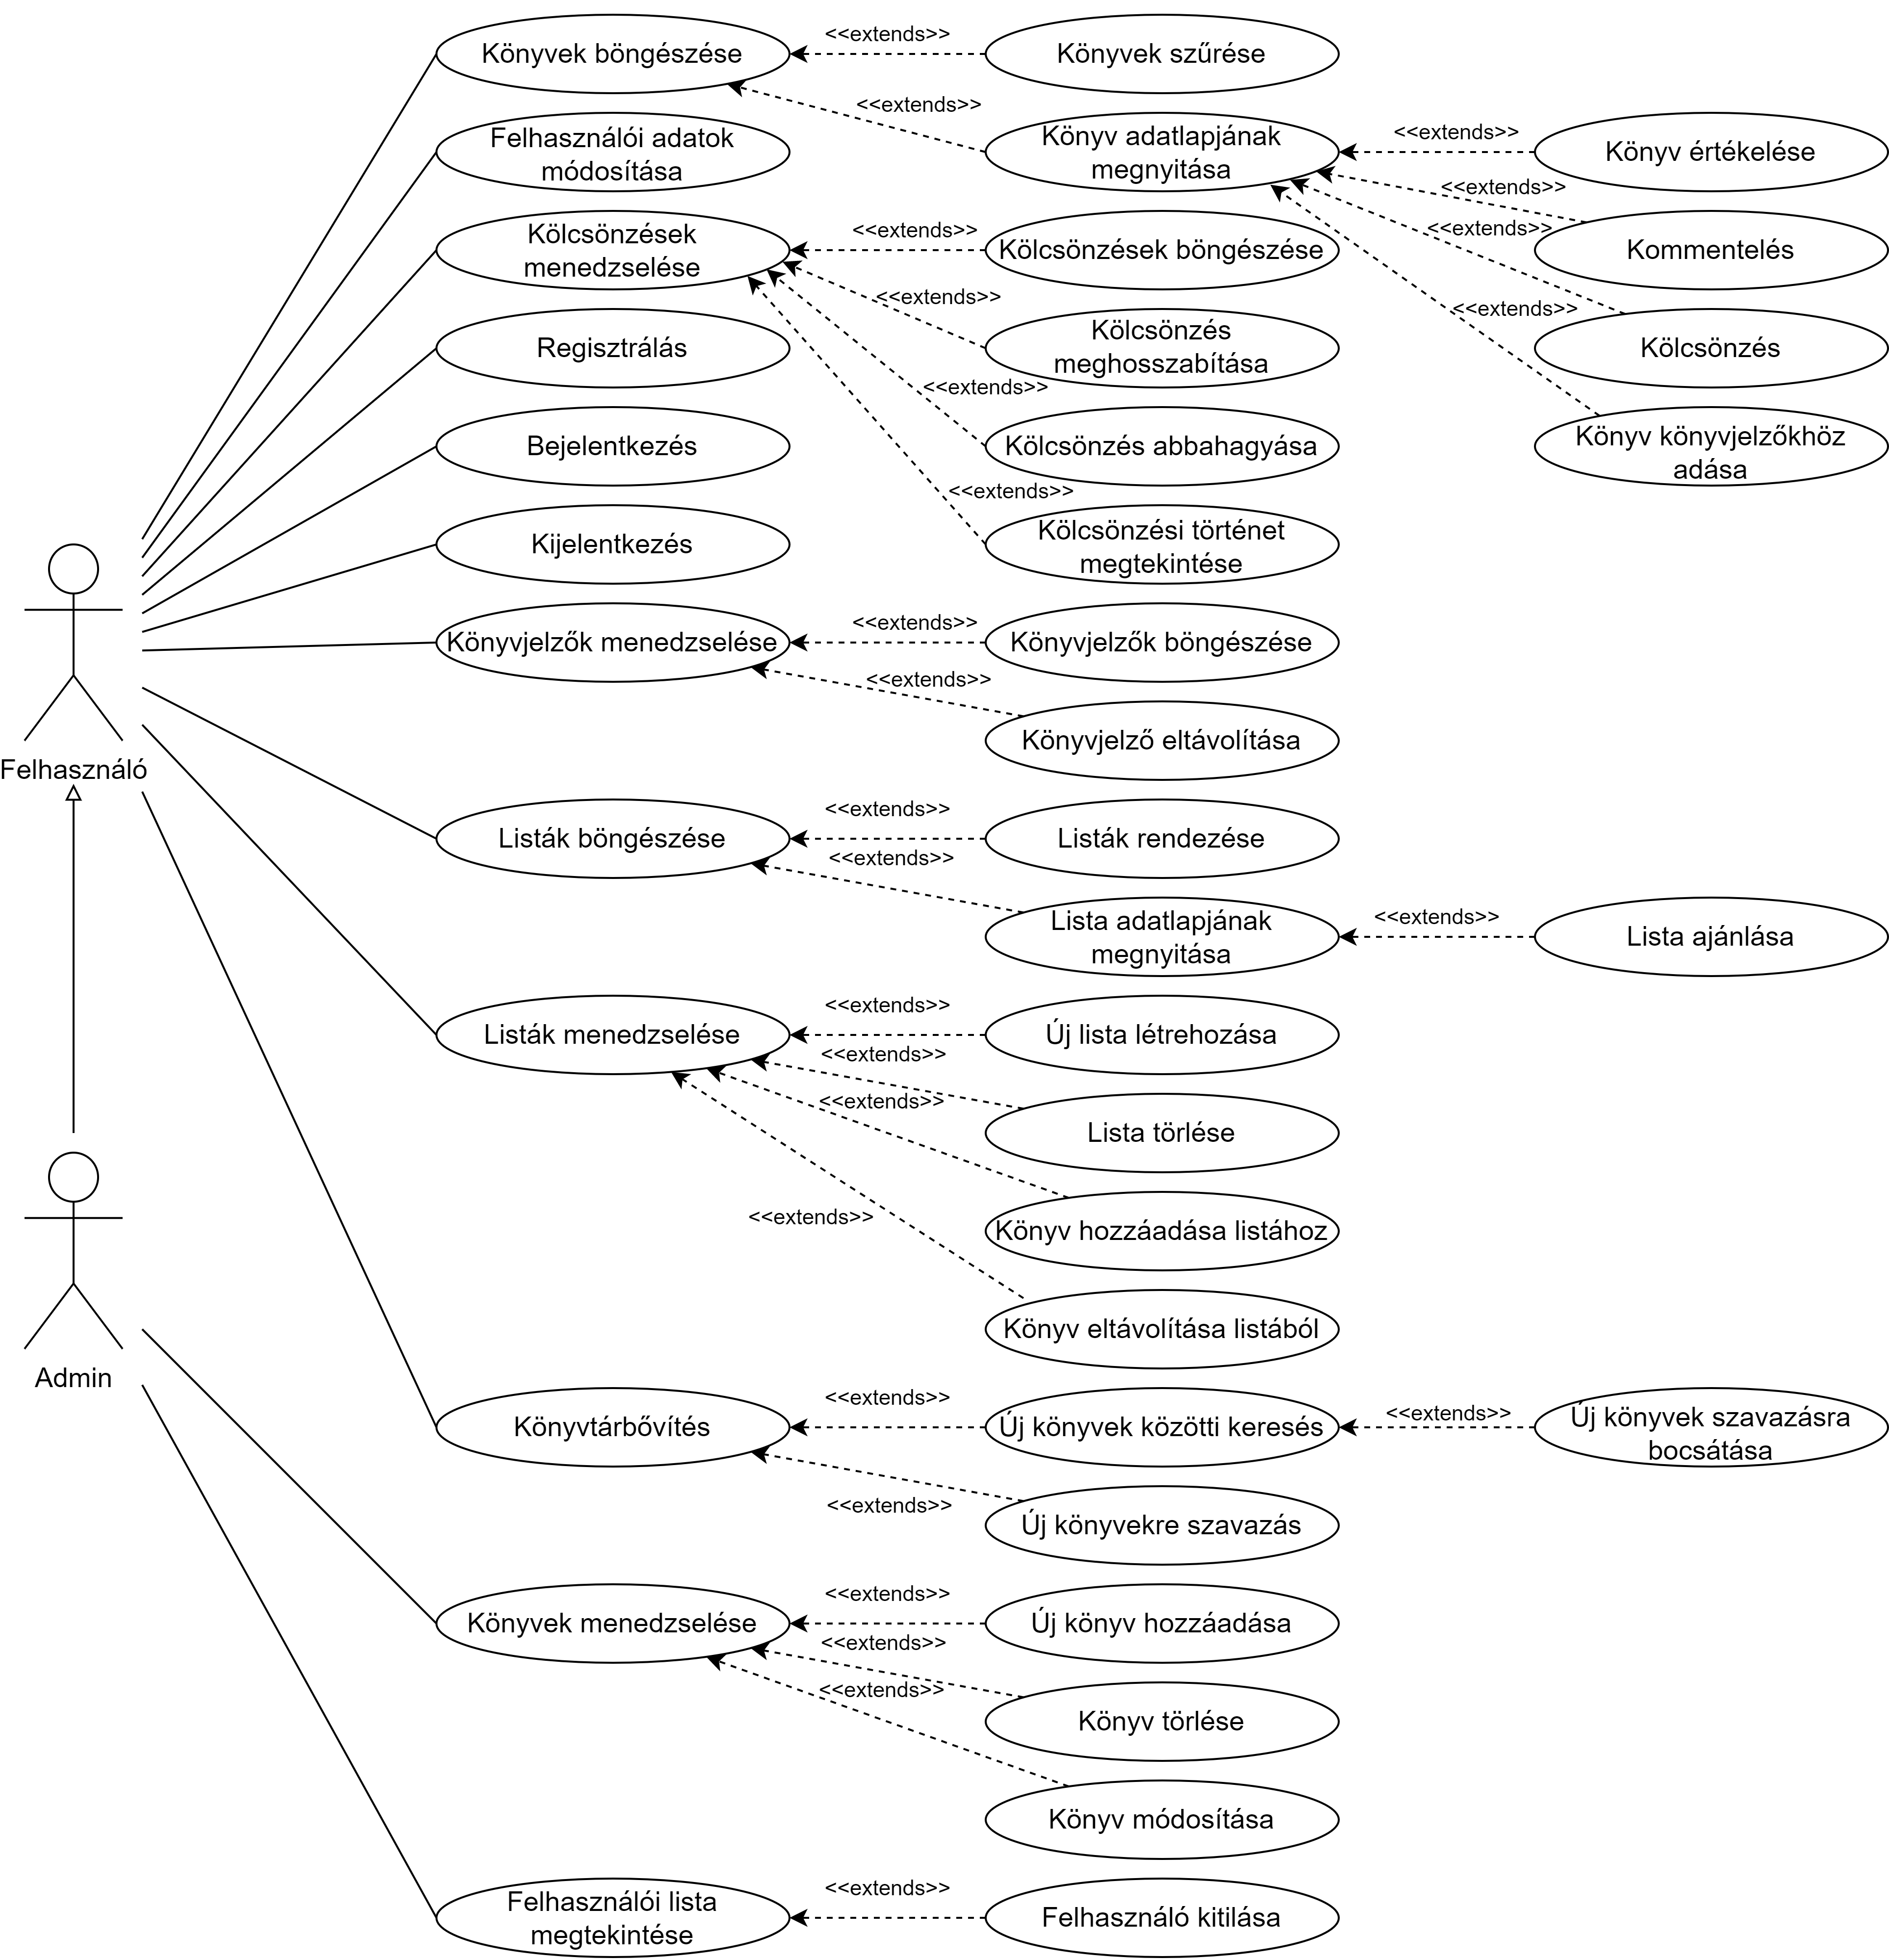
\includegraphics[scale=0.6]{images/graphlibrary-usecase-better.png}
	\caption{Az alkalmazás használati esetei}
	\label{fig:use-case}
\end{figure}

Egy átlagos felhasználó az alkalmazásban az alábbiakban felsorolt funkciókat tudja igénybe venni.
\begin{itemize}
    \item Felhasználói fiókkal kapcsolatos funkciók: regisztrálás, bejelentkezés, kijelentkezés, felhasználói adatok módosítása.
    \item Könyvkereséssel kapcsolatos funkciók: könyvek böngészése, könyvek szűrése, \\ könyvek adatlapjának megnyitása.
    \item A könyvek adatlapján igénybe vehető funkciók: könyvek értékelése, megjegyzés írása, könyv kikölcsönözése, könyv könyvjelzőkhöz adása, könyv eltávolítása.
    \item Kölcsönzésekkel kapcsolatos funkciók: kölcsönzések böngészése, kölcsönzések \\ meghosszabbítása, könyvek visszavitele, felhasználó kölcsönzési történetének \\ megtekintése.
    \item Könyvjelzőkkel kapcsolatos funkciók: könyvjelzők böngészése, könyvjelzők eltávolítása.
    \item Listák böngészésével kapcsolatos funkciók: listák böngészése, rendezése, listák adatlapjának megtekintése, listák ajánlása.
    \item Saját listákkal kapcsolatos funkciók: új lista létrehozása, lista törlése, könyv listához adása, könyv eltávolítása a listából.
    \item Könyvtárbővítéssel kapcsolatos funkciók: lehetséges könyvek közötti keresés, azok szavazásra bocsátása, szavazatra bocsátott könyvekre szavazás.
\end{itemize}

Adminisztrátori jogosultságú felhasználó az alkalmazásban az alábbi funkciókat tudja igénybe venni.
\begin{itemize}
    \item Felhasználókkal kapcsolatos funkciók: felhasználói lista megtekintése, felhasználók kitiltása.
    \item Könyvekkel kapcsolatos funkciók: új könyv könyvtárhoz adása, meglévő könyvek módosítása, könyvek törlése.
\end{itemize}

\Section{Funkciók, műveletek}

% TODO: Itt már részletesebben ki lehet fejteni a kölcsönzést, a listázásokat, az értékelést.

Ebben az alfejezetben bemutatásra kerül, hogy milyen funkciókkal van felruházva a mintaalkalmazás. A bemutatás az alkalmazás menüpontjain keresztül fog zajlani.

\subsection{Books menüpont}

A \textit{Books} menüpont az alkalmazás központi része (\ref{fig:books}. ábra). Innen érheti el a felhasználó a könyvtárban található könyvek adatait. A menüpont megnyitásakor az oldal közepén megjelennek a könyvtárban található könyvek. Egyszerre csak egy adott számú könyv jelenik meg, további könyveket a találatok alatt lévő lapszámozás funkció segítségével lehet elérni. A nyilakra kattintva egy-egy oldallal az adott irányba lehet lépni, míg egy adott számra kattintva az azzal megegyező sorszámú találatoldal fog megjelenni.

\begin{figure}[h]
\centering
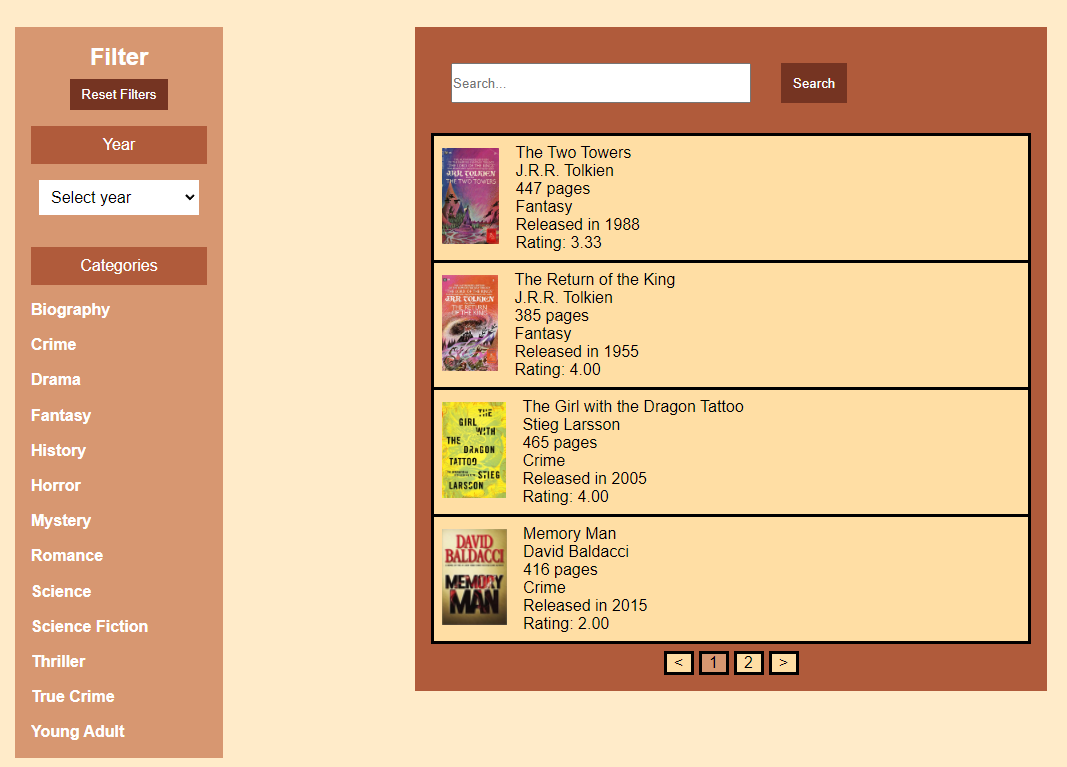
\includegraphics[scale=0.5]{images/application/books.png}
\caption{A Books menüpont}
\label{fig:books}
\end{figure}

A megjelenő könyveket lehetősége van a felhasználónak szűrni. A könyvek felett található keresési mezőbe beírhatja a felhasználó egy könyv címét, vagy címének egy részletét, és ekkor csak a keresésnek megfelelő könyvek fognak megjelenni a listában. Ezen kívül lehetősége van még a felhasználónak a könyvektől balra található felületen megjelenési év, valamint kategória szerint is szűrni a találatokat. Ez a három szűrési lehetőség egyszerre is használható.

Minden megjelenő könyvhöz tartozik egy rövid összefoglaló. Ebben az összefoglalóban megtudhatja a felhasználó az adott könyv címét, a szerzőjét, oldalainak számát, kategóriáját, megjelenési évét, borítója, valamint a más felhasználók értékelésének átlagát. Egy összefoglalóra kattintva megjelenik az adott könyv adatlapja (\ref{fig:bookcard}. ábra).

Egy könyv adatlapját megnyitva megjelennek a könyv adatai, úgy mint: 
\begin{itemize}
    \item cím,
    \item szerző(k),
    \item rövid tartalmi összefoglaló,
    \item hossz,
    \item kategória,
    \item megjelenési év,
    \item értékelések átlaga,
    \item könyvtári példányok száma.
\end{itemize}

\begin{figure}[h]
    \centering
    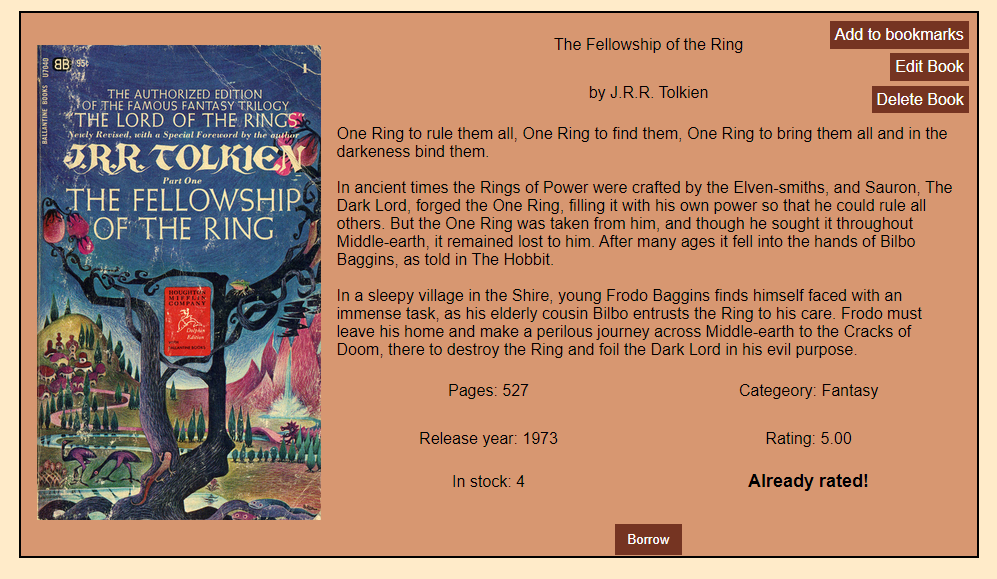
\includegraphics[scale=0.55]{images/application/bookcard.png}
    \caption{Egy könyv adatlapja}
    \label{fig:bookcard}
\end{figure}

Az adatlap alatt más felhasználók által írt kommenteket találhat a felhasználó. Egy kommentnél az alábbi információk jelennek meg:
\begin{itemize}
    \item a kommentelő neve,
    \item a komment írásának dátuma,
    \item a komment szöveges tartalma.
\end{itemize}
Bejelentkezés nélkül a felhasználónak csak az adatlap megtekintésére van lehetősége. Egy bejelentkezett felhasználó számára az alábbi funkciók is elérhetővé válnak.
\begin{itemize}
    \item Az értékelések alatt lehetősége van egy regisztrált felhasználónak a könyv értékelésére 1 és 5 közötti értékkel.
    \item  Az adatlap jobb felső sarkában a felhasználó a könyvjelzőihez adhatja a könyvet, vagy ha már ott volt, akkor eltávolíthatja azt onnan.
    \item  Az adatlap alján lehetősége van a felhasználónak az adott könyv kikölcsönzésére, amennyiben a könyv készleten van.
    \item  Az adatlap alatt írhat saját kommentet is a felhasználó.
\end{itemize}
Admin jogosultsággal rendelkező felhasználónak a könyv adatlapról lehetősége van még ezeken kívül a könyvet szerkeszteni, illetve törölni.

\subsection{Lists menüpont}

A \textit{Lists} menüpontban lehetősége van a felhasználónak más felhasználók által készített listák megtekintésére, valamint saját listák menedzselésére.

A \textit{Browse Lists} almenüpontra kattintva megjelennek a felhasználók által készített listák. A \textit{Books} menüponthoz hasonlóan itt a lapszámozás funkció segítségével válthat a felhasználó a listák között. A listákat lehetősége van a felhasználónak ajánlások, illetve létrehozási dátum szerint rendezni. Minden listához tartozik egy összefoglaló, ami az alábbiakat tartalmazza:
\begin{itemize}
    \item a lista neve,
    \item a listában levő könyvek száma,
    \item az ajánlások száma,
    \item a lista létrehozásának dátuma.
\end{itemize}
Egy lista összefoglalójára kattintva megjelenik a lista adatlapja (\ref{fig:listcard}. ábra).

\begin{figure}[h]
    \centering
    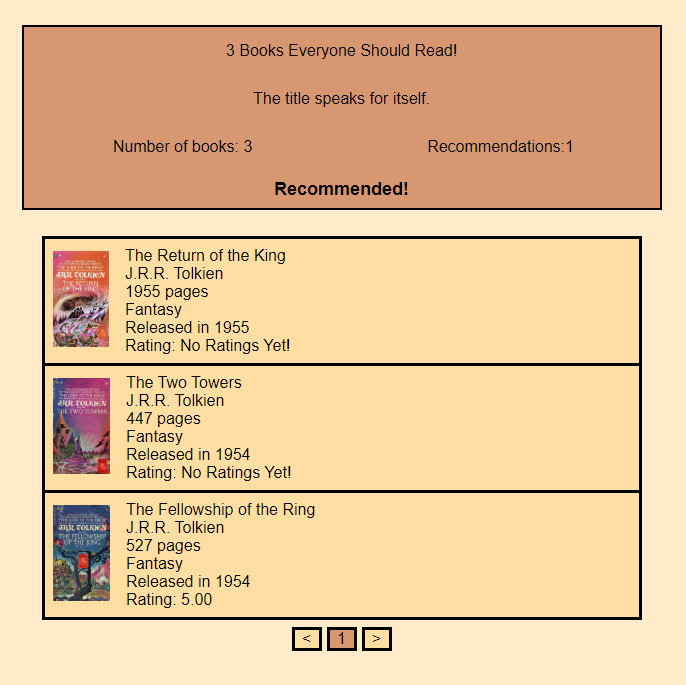
\includegraphics[scale=0.65]{images/application/listcard.png}
    \caption{Egy lista adatlapja}
    \label{fig:listcard}
\end{figure}

\noindent A lista adatlapján az alábbiak szerepelnek:
\begin{itemize}
    \item a lista neve,
    \item a lista leírása,
    \item listában levő könyvek száma,
    \item az ajánlások száma.
\end{itemize}

Az adatlap alatt láthatja a felhasználó, hogy pontosan mely könyvek vannak a listában. Bejelentkezett felhasználónak lehetősége van a lista ajánlására.

A \textit{New List} menüpontban a felhasználó egy listanév és egy leírás megadásával saját listát hozhat létre. A felhasználó a saját listáit a \textit{Delete List} menüpontban törölheti.

Az \textit{Add Books To List} menüpontban lehetősége van a felhasználónak kiválasztania egyet a listái közül. Egy lista kiválasztása utána a \textit{Books} menüpont felülete jelenik meg annyi különbséggel, hogy minden könyv elemhez tartozik egy \textit{Add} gomb, amivel az adott könyv a listához rendelhető. A \textit{Remove Book From List} menüpontban a lista kiválasztása után megjelennek a listához tartozó könyvek, melyeket a \textit{Remove} gombra kattintva lehet eltávolítani az adott listából.

\subsection{Expand menüpont}

Az \textit{Expand} menüpont lehetőséget nyújt a felhasználók számára, hogy a könyvtárban még nem található könyvekkel bővítsék a könyvtár készletét. 

Az \textit{Add} almenüpontban lehetősége van a felhasználónak cím, író és kategória szerint keresni a Google Books katalógusában. Keresés után megjelennek a találatok, melyekhez tartozik egy-egy rövid összefoglaló, amely az alábbi adatokat tartalmazza:
\begin{itemize}
    \item cím,
    \item író,
    \item oldalszám,
    \item kategória,
    \item megjelenési év,
    \item tartalmi összegzés (kattintás után).
\end{itemize}
Minden találathoz tartozik egy \textit{Add} gomb, amire ha rákattint a felhasználó, akkor a könyv szavazásra bocsátásra kerül.

A \textit{Vote} almenüpontban lehetősége van a felhasználónak szavazásra bocsátott könyvekre szavazni. Ha egy könyv elég szavazatot gyűjt, akkor az hozzáadódik a könyvtárhoz (\ref{fig:expand}. ábra).

\begin{figure}[h]
    \centering
    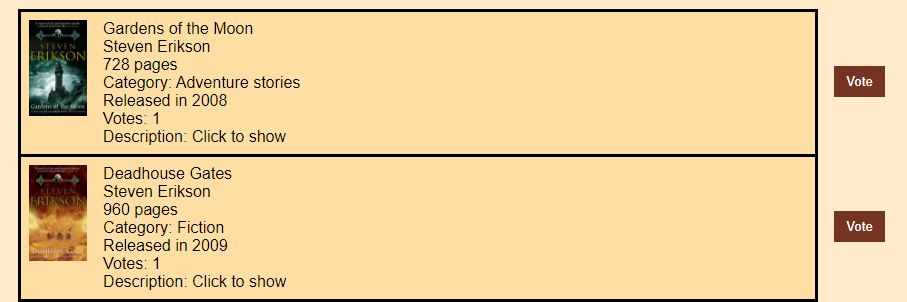
\includegraphics[scale=0.6]{images/application/expand.png}
    \caption{Bővítés menüpont -- Szavazás funkció}
    \label{fig:expand}
\end{figure}

\subsection{Borrowings menüpont}

A \textit{Borrowings} menüpontban tudja a felhasználó megtekinteni a jelenlegi kölcsönzéseit. A könyvek a rövid összefoglaló formájukban jelennek meg. Minden megjelenő könyvtől jobbra találhatóak a kölcsönzéssel kapcsolatos információk, illetve lehetőségek (\ref{fig:borrowings}. ábra). 

\begin{figure}[h]
    \centering
    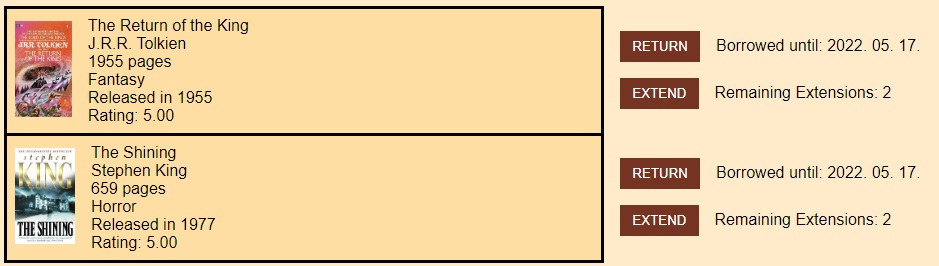
\includegraphics[scale=0.6]{images/application/borrowings.png}
    \caption{Kölcsönzések menüpont}
    \label{fig:borrowings}
\end{figure}

Egy könyv kikölcsönzése alapvetően 30 napra szól. Ezt az időtartamot a felhasználónak kétszer van lehetősége meghosszabbítani, mindegyik hosszabbítás 30 napot ad a teljes időtartamhoz, tehát egy felhasználó egy könyvet maximum 90 napig tarthat magánál. Azt, hogy hány hosszabbítási lehetősége van a felhasználónak, és hogy meddig tart a kölcsönzési határidő, a könyvtől jobbra található részen láthatja a felhasználó. Az \textit{Extend} gombra kattintva megtörténik a hosszabbítás, a \textit{Return} gombra kattintva pedig a felhasználó visszaadja a könyvet a könyvtárnak. 

\subsection{Bookmarks menüpont}

A \textit{Bookmarks} menüpontban megtekintheti a felhasználó a könyvjelzőit. A könyvek a rövid összefoglaló formájukban jelennek meg. Minden könyvhöz tartozik egy \textit{Remove} gomb, amivel a felhasználó eltávolíthatja a könyvet a könyvjelzők közül (\ref{fig:bookmarks}. ábra).

\begin{figure}[h]
    \centering
    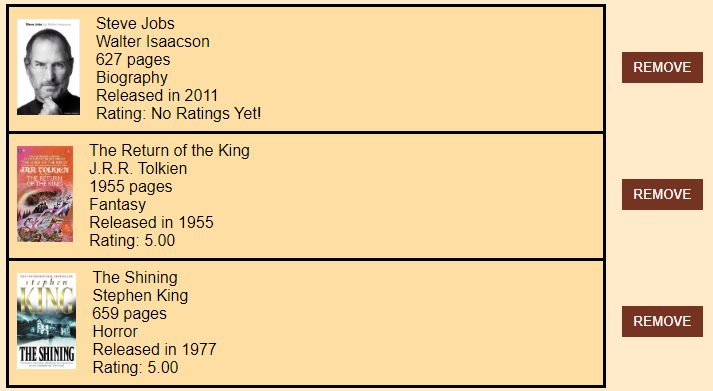
\includegraphics[scale=0.65]{images/application/bookmarks.png}
    \caption{Könyvjelzők menüpont}
    \label{fig:bookmarks}
\end{figure}

\subsection{Signup menüpont}

A \textit{Signup} menüpontban hozhat létre a felhasználó saját felhasználói fiókot. Egy ilyen fiók szükséges ahhoz, hogy az alkalmazás funkcióinak többsége igénybe vehető legyen. A regisztrációhoz meg kell adni egy nevet, egy egyedi email címet és egy jelszót. Már foglalt email cím megadása esetén a felhasználó hibaüzenetet kap.

\subsection{Login menüpont}

A \textit{Login} menüpontban léphet be a felhasználó a létrehozott felhasználói fiókjába helyes email cím és jelszó kombináció megadása után. Hibás bejelentkezési adatok esetén a felhasználó hibaüzenetet kap.

\subsection{Profile menüpont}

A \textit{History} gombra kattintva megtekintheti a felhasználó, hogy milyen korábbi kölcsönzései voltak.

A \textit{Change User Data} gombra kattintva lehetősége van a felhasználónak a nevét, jelszavát és/vagy email címét megváltoztatni a jelenlegi jelszó megadása után. Hibás adatok esetén a felhasználó hibaüzenetet kap.

\subsection{Admin menüpont}

Az \textit{Admin} menüponthoz csak az adminisztrátor jogosultsággal rendelkező felhasználóknak van hozzáférési joga. 

Az \textit{Add New Book} gombra kattintva megjelenik egy űrlap, amelyen meg tudja adni az adminisztrátor az új könyv címét, szerzőjét, rövid tartalmi összegzését, hosszát, kategóriáját, megjelenési évét, borítóját, és hogy hány darab van a könyvből készleten. Az \textit{Add Book} gombra kattintva az űrlapon megadott könyv hozzáadódik a könyvtárhoz (\ref{fig:newbook}. ábra).

\begin{figure}[h]
    \centering
    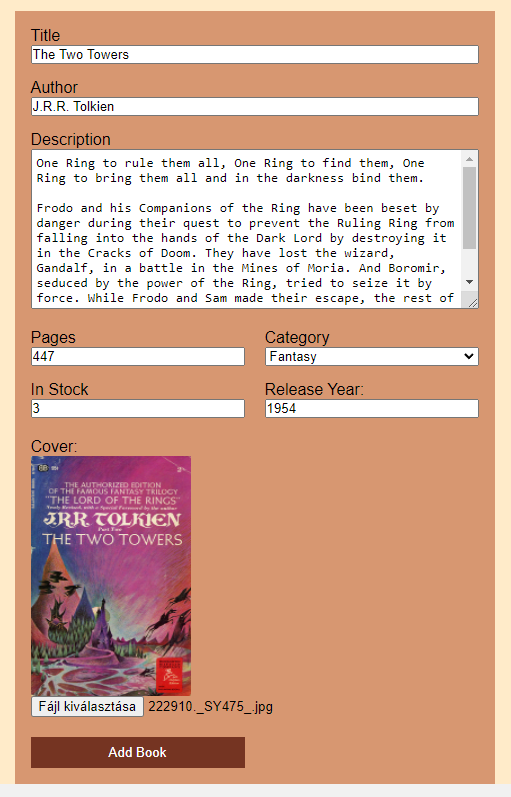
\includegraphics[scale=0.7]{images/application/newbook.png}
    \caption{Új könyv hozzáadása}
    \label{fig:newbook}
\end{figure}

A \textit{User List} gombra kattintva megjelenik az összes felhasználó neve és email címe (\ref{fig:userlist}. ábra). A \textit{Ban user} gombra kattintva lehetősége van az adminisztrátornak egy felhasználó végleges kitiltására.

\begin{figure}[h]
    \centering
    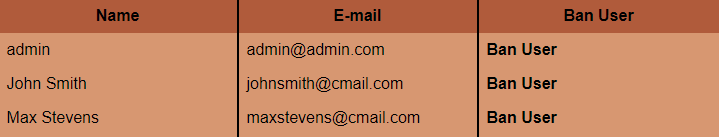
\includegraphics[scale=0.7]{images/application/userlist.png}
    \caption{Felhasználói lista}
    \label{fig:userlist}
\end{figure}

\Section{Az alkalmazás architektúrája}

% TODO: Ide kellene egy áttekintő jellegű ábra az "elkészítendő" alkalmazás szerkezetéről. Ez mutatná be, hogy a felhasznált technológiák hogyan kapcsolódnak egymáshoz.

Az alkalmazás architektúrájának fő elemeit \aref{fig:graphlibrary_architecture}. ábra foglalja össze.

\begin{figure}[h]
   \centering
   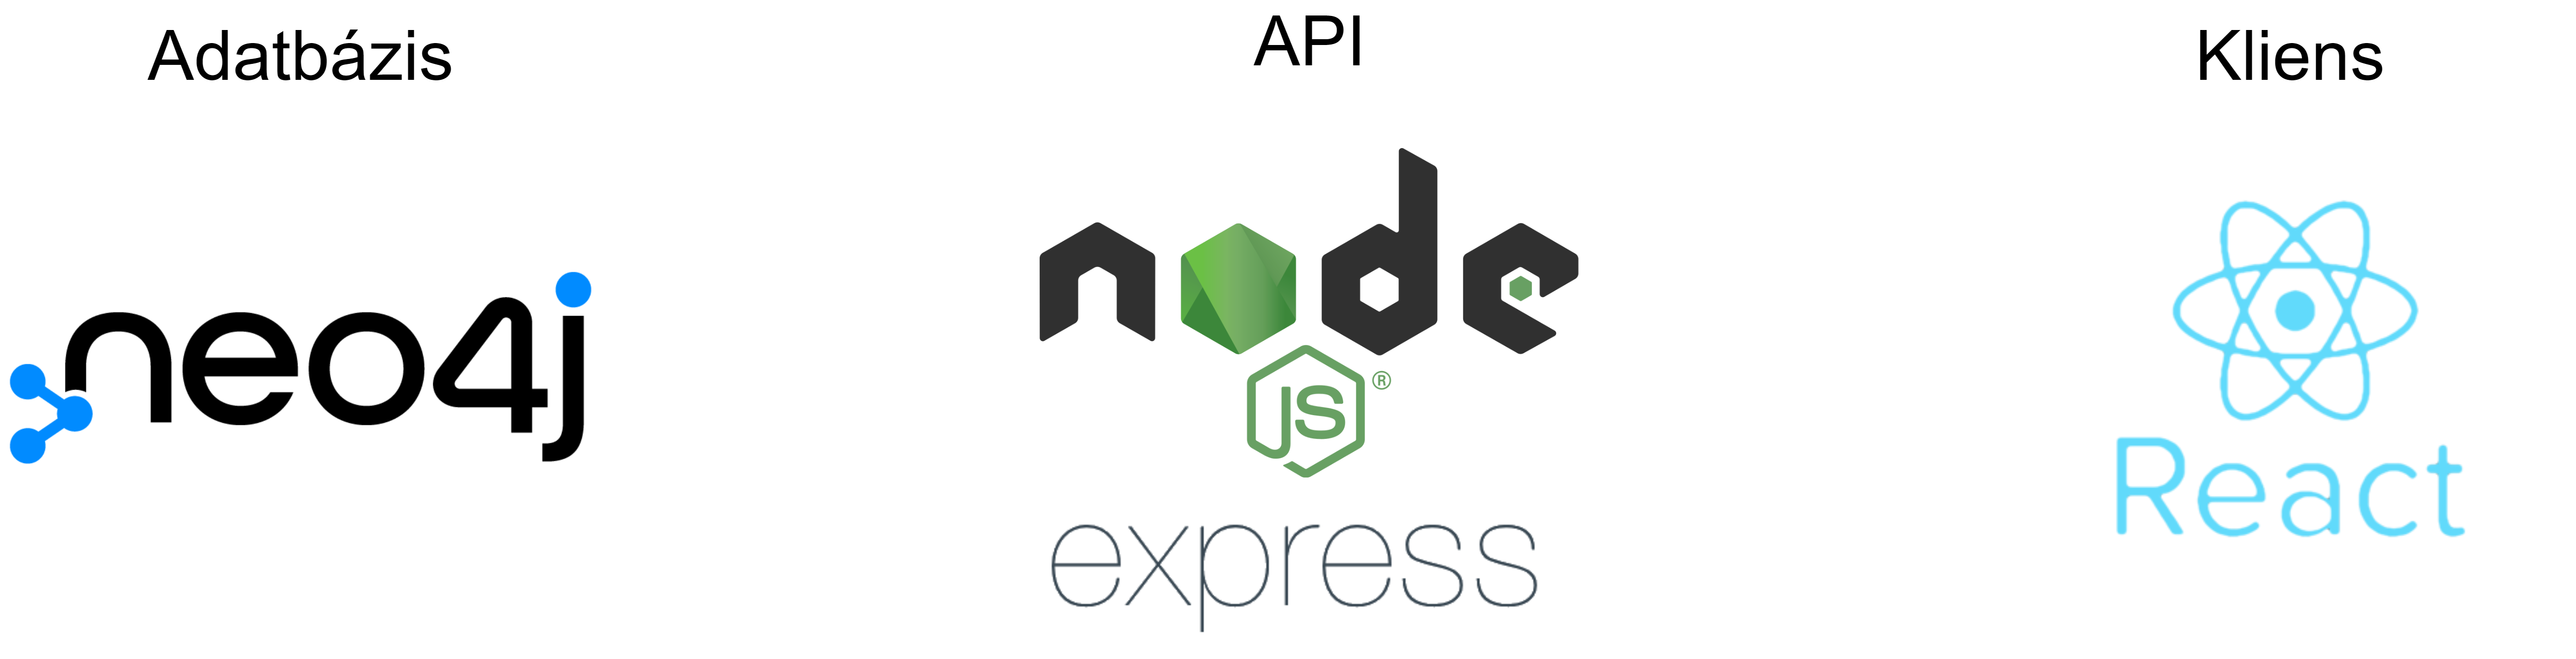
\includegraphics[scale=0.3]{images/graphlibrary_architecture.png}
   \caption{Az alkalmazás architektúrájának sematikus ábrája}
   \label{fig:graphlibrary_architecture}
\end{figure}

A kliens a React könyvtár segítségével valósul meg. Az adatok a Neo4j gráfadatbázisban kerülnek tárolásra. A kettő közötti kommunikációt a NodeJS és az Express keretrendszer teszi lehetővé.

\Section{Az alkalmazás API-ja}

Ebben az alfejezetben található az API tömör leírása. Az API részletes, OpenAPI szabvány szerinti leírása külön (a \texttt{graph-library-api.yaml}) fájlban olvasható.

A tervezés során szempont volt a REST architekturális stílus alkalmazása. A következőkben az API bemutatásánál a jellegzetességekre, döntési pontok indoklására kerül majd sor. (Az egyszerűbb, következetesen adódó esetek különösebb részletezése nem tünt szükségesnek.)

\subsection{Könyvekkel kapcsolatos operációk}

\Aref{tab:book}. táblázatban láthatjuk a könyvekhez kapcsolódó műveleteket. Ennek egy érdekesebb pontja több könyv adatainak visszaadása az azonosítók alapján. Ez egy GET típusú kérés, amelynél viszont paraméterként szerepelnie kell a könyvek azonosítóinak listájának. Mivel az egyidejűleg lekérdezésre kerülő könyvek száma lehetővé tette, ezért ez az útvonalban került megadásra.

\renewcommand\tabularxcolumn[1]{m{#1}}
\begin{center}
\begin{table}[h]
\caption{Book operációk}
\label{tab:book}
\smallskip
\begin{tabularx}{\textwidth}{ |l|c|Y|Y| } 
 \hline
 \multicolumn{1}{|c|}{\texttt{Útvonal}} & \texttt{Metódus} & \texttt{Paraméterek} & \texttt{Feladat} \\ 
 \hhline{|=|=|=|=|}
 /book & POST & Könyv objektum & Új könyv létrehozása  \\ 
 \hline
 /book & GET & Keresési feltételek, Pagination adatok & Könyvek visszaadása  \\ 
 \hline
 /book & DELETE & Könyv ID & Könyv törlése  \\ 
 \hline
 /book & PUT & Könyv objektum & Könyv módosítása  \\ 
 \hline
 /book/list/\{listOfIds\} & GET & Könyv ID-k listája, Pagination adatok & Könyvek visszaadása  \\ 
 \hline
 /book/\{bookId\} & GET & Könyv ID & ID-nek megfelelő könyv visszaadása  \\ 
 \hline
 /book/rate & POST & Könyv és Felhasználó ID, Értékelés & Új értékelés hozzáadása  \\ 
 \hline
\end{tabularx}
\end{table}
\end{center}

\subsection{Kommentekkel kapcsolatos operációk}

A kommentekhez kapcsolódó műveleteket \aref{tab:comment}. táblázatban láthatjuk. Mivel a megjegyzések utólagos szerkesztésére a rendszer (az aktuális változat tervei szerint) nem ad lehetőséget, ezért elegendő volt csak a könyvhöz tartozó kommentek lekérdezését és új komment létrehozását biztosítani az API-n keresztül.

\begin{center}
\begin{table}[h]
\caption{Comment operációk}
\label{tab:comment}
\smallskip
\begin{tabularx}{\textwidth}{ |l|c|Y|Y| } 
 \hline
 \multicolumn{1}{|c|}{\texttt{Útvonal}} & \texttt{Metódus} & \texttt{Paraméterek} & \texttt{Feladat} \\ 
 \hhline{|=|=|=|=|}
 /comment/\{bookId\} & GET & Könyv ID & Könyvhöz tartozó kommentek visszaadása  \\ 
 \hline
 /comment & POST & Komment objektum & Új komment létrehozása  \\ 
 \hline
\end{tabularx}
\end{table}
\end{center}

\subsection{Listákkal kapcsolatos operációk}

A listákhoz tartozó műveleteket \aref{tab:list}. táblázat foglalja össze. A könyvekhez és kommentekhez hasonlóan, az API nem teljes körű olyan tekintetben, hogy például az ajánlásokhoz nem biztosít minden CRUD műveletet. Ez ez esetben sem következetlenség, hanem a specifikált funkcionalitás nem tette szükségessé ezen végpontok kialakítását.

\begin{center}
\begin{table}[h]
\caption{List operációk}
\label{tab:list}
\smallskip
\begin{tabularx}{\textwidth}{ |l|c|Y|Y| } 
 \hline
 \multicolumn{1}{|c|}{\texttt{Útvonal}} & \texttt{Metódus} & \texttt{Paraméterek} & \texttt{Feladat} \\ 
 \hhline{|=|=|=|=|}
 /list & POST & Lista objektum & Új lista létrehozása  \\ 
 \hline
 /list & GET & Pagination információk, Rendezési sorrend & Lista visszaadása  \\ 
 \hline
 /list & DELETE & Lista ID & Lista törlése  \\ 
 \hline
 /list/user/\{userId\} & GET & Felhasználó ID & Felhasználó listáinak visszaadása  \\ 
 \hline
 /list/\{listId\} & GET & Könyv objektum & ID-nek megfelelő lista visszaadása  \\ 
 \hline
 /list/book & POST & Könyv ID, Lista ID & Könyv listához adása  \\ 
 \hline
 /list/book & DELETE & Könyv ID, Lista & Könyv törlése listából  \\ 
 \hline
 /list/recommendation & POST & Lista ID & Új ajánlás hozzáadása  \\ 
 \hline
\end{tabularx}
\end{table}
\end{center}

\subsection{Bővítéssel kapcsolatos operációk}

A könyvállomány bővítéséhez kapcsolódó műveleteket \aref{tab:expand}. táblázatban láthatjuk. Ez egyúttal tartalmazza a szavazáshoz szükséges végpontot is.

\begin{center}
\begin{table}[H]
\caption{Expand operációk}
\label{tab:expand}
\smallskip
\begin{tabularx}{\textwidth}{ |l|c|Y|Y| } 
 \hline
 \multicolumn{1}{|c|}{\texttt{Útvonal}} & \texttt{Metódus} & \texttt{Paraméterek} & \texttt{Feladat} \\ 
 \hhline{|=|=|=|=|}
 /expand & POST & Könyv objektum, Felhasználó ID & Új potenciális könyv létrehozása  \\ 
 \hline
 /expand & GET & Pagination információk & Potenciális könyvek visszaadása  \\ 
 \hline
 /expand & DELETE & Könyv ID & Potenciális könyv eltávolítása  \\ 
 \hline
 /expand/vote & POST & Könyv ID, Felhasználó ID & Új szavazás hozzáadása  \\ 
 \hline
\end{tabularx}
\end{table}
\end{center}

\subsection{Kölcsönzésekkel kapcsolatos operációk}

A kölcsönzés esetében \aref{tab:borrow}. táblázatban látható műveletek érhetők el. A kölcsönzést leíró objektum átadása esetén a felhasználói azonosítónak nem szükséges szerepelnie az útvonalban.

\begin{center}
\begin{table}[h]
\caption{Borrow operációk}
\label{tab:borrow}
\smallskip
\begin{tabularx}{\textwidth}{ |l|c|Y|Y| }
 \hline
 \multicolumn{1}{|c|}{\texttt{Útvonal}} & \texttt{Metódus} & \texttt{Paraméterek} & \texttt{Feladat} \\ 
 \hhline{|=|=|=|=|}
 /borrow/\{userId\} & GET & Felhasználó ID & Felhasználó kölcsönzéseinek visszaadása\\ 
 \hline
 /borrow & POST & Kölcsönzés objektum & Új Kölcsönzés létrehozása  \\ 
 \hline
 /borrow & DELETE & Kölcsönzés objektum & Kölcsönzés törlése \\ 
 \hline
 /borrow/extend & POST & Kölcsönzés objektum & Kölcsönzés meghosszabbítása \\ 
 \hline
\end{tabularx}
\end{table}
\end{center}

\pagebreak

\subsection{Könyvjelzőkkel kapcsolatos operációk}

A könyvjelzők műveleteinek áttekintését \aref{tab:bookmarks}. táblázatban láthatjuk. A törlésnél elegendő volt csak a könyvet átadni paraméterként, mivel abból egyértelműen azonosítható a könyvjelző objektum is.

\begin{center}
\begin{table}[h]
\caption{Bookmarks operációk}
\label{tab:bookmarks}
\smallskip
\begin{tabularx}{\textwidth}{ |l|c|Y|Y| } 
 \hline
 \multicolumn{1}{|c|}{\texttt{Útvonal}} & \texttt{Metódus} & \texttt{Paraméterek} & \texttt{Feladat} \\ 
 \hhline{|=|=|=|=|}
 /bookmarks/\{userId\} & GET & Felhasználó ID & Felhasználó könyvjelzőinek visszaadása\\ 
 \hline
 /bookmarks & POST & Könyvjelző objektum & Új könyvjelző létrehozása  \\ 
 \hline
 /bookmarks & DELETE & Könyv objektum & Könyvjelző törlése \\ 
 \hline
\end{tabularx}
\end{table}
\end{center}

\subsection{Felhasználókkal kapcsolatos operációk}

A felhasználók kezeléséhez tartozó műveleteket \aref{tab:user}. táblázat foglalja össze. A módosítással és törléssel kapcsolatos adatok a POST és a PUT kérés paramétereibe kerültek. Alternatívaként felvetődött a felhasználói azonosító útvonalban történő megadása is.

\begin{center}
\begin{table}[h]
\caption{User operációk}
\label{tab:user}
\smallskip
\begin{tabularx}{\textwidth}{ |l|c|Y|Y| } 
 \hline
 \multicolumn{1}{|c|}{\texttt{Útvonal}} & \texttt{Metódus} & \texttt{Paraméterek} & \texttt{Feladat} \\ 
 \hhline{|=|=|=|=|}
 /user & POST & Felhasználó objektum & Új felhasználói fiók létrehozása  \\ 
 \hline
 /user & GET & - & Felhasználók visszaadása  \\ 
 \hline
 /user & PUT & Felhasználó objektum & Felhasználó módosítása  \\ 
 \hline
 /user & DELETE & Felhasználó ID & Felhasználói fiók törlése  \\ 
 \hline
 /user/login & POST & Bejelentkezési adatok & Felhasználói fiókba való bejelentkezés \\ 
 \hline
\end{tabularx}
\end{table}
\end{center}

\subsection{Kölcsönzési történettel kapcsolatos operációk}

\Aref{tab:historyborrow}. táblázat a kölcsönzés naplózásához szükséges API végpontok rövid áttekintését mutatja be. Az ehhez tartozó bejegyzések módosítása és törlése nem tünt szükségesnek, így az API kifejezetten egyszerű tudott maradni.

\begin{center}
\begin{table}[h]
\caption{Historyborrow operációk}
\label{tab:historyborrow}
\smallskip
\begin{tabularx}{\textwidth}{ |l|c|Y|Y| } 
 \hline
 \multicolumn{1}{|c|}{\texttt{Útvonal}} & \texttt{Metódus} & \texttt{Paraméterek} & \texttt{Feladat} \\ 
 \hhline{|=|=|=|=|}
 /historyborrow & POST & Felhasználó ID, Könyv ID, Dátum & Kölcsönzés naplózása  \\ 
 \hline
 /historyborrow/\{userID\} & GET & Felhasználó ID, Pagination információk & Kölcsönzése történet visszaadása  \\ 
 \hline
\end{tabularx}
\end{table}
\end{center}

\Section{A kliens alkalmazás}
% TODO: Be kellene mutatni, hogy a kliens milyen nagyobb részekből épül fel. Az implementáció
%Általános React információk, alapvető kliens felépítés, információk

% https://hu.reactjs.org/tutorial/tutorial.html#what-is-react idézet:
A kliens alkalmazás a React JavaScript függvénykönyvtárral valósul meg \cite{react}. Ez lehetőséget ad az elemek deklaratív leírására. Komponens alapú szemléletet követ, amellyel így a nagyobb méretű alkalmazások fejlesztése esetében is kezelhető marad a kódbázis.

% "A React egy deklaratív, effektív, és rugalmas JavaScript könyvtár, felhasználói felületek készítéséhez. Lehetővé teszi komplex felhasználói felületek összeállítását izolált kódrészletekből, amiket “komponenseknek” hívunk." \cite{react}

A komponensek közötti adatcsere property-kkel (úgynevezett \textit{prop}-okkal) valósul meg, például:
\begin{java}
<BookItem
  title={"The Fellowship of the Ring"}
  author={"J.R.R. Tolkien"}
/>
\end{java}
Ebben a példában a \texttt{BookItem} komponens két prop-ot kap (\texttt{title} és \texttt{book}), amiket a komponens később fel tud használni. Ahhoz, hogy ezek elérhetők legyenek, a komponens deklarációjakor be kell állítani, hogy fogadjon propokat:
\begin{java}
const BookItem = (props) => {...}
\end{java}
Ez után például a \texttt{title} prop értékét meg lehet kapni a \texttt{props.title} formában.

Az alkalmazás inicializálása a \texttt{create-react-app} eszközzel történik, aminek a lépései a következők Node package manager esetében:
\begin{itemize}
    \item \texttt{npm install -g create-react-app} parancs futtatása, ami telepíti az eszközt
    \item \texttt{npm init react-app my-app} parancs futtatása, ami inicializálja a React alkalmazást
    \item \texttt{npm start} parancs futtatása, ami elindítja az alkalmazást
\end{itemize}

A \texttt{useState} React Hook segítségével deklarálhatunk úgynevezett állapot változókat. Ezek olyan változók, amelyek a komponens újrarajzolásakor nem veszítik el értéküket. Például:
\begin{java}
const [book, setBook]=useState("The Fellowship of the Ring")
\end{java}
Itt a \texttt{book} a változó, aminek kezdőértéke a "\textit{The Fellowship of the Ring}" sztring. A változó értékét a \texttt{setBook} függvénnyel lehet megváltoztatni:
\begin{java}
setBook("The Two Towers")
\end{java}
Ezzel a változó értéke a "The Two Towers" sztringre változik. A változó értékének változásakor a komponens ez esetben is újrarajzolódik.

%useeffect, cleanup
\begin{java}
useEffect(() => {
  getBook(bookId).then((data) => {
    setBook(data);
  });
}, [bookId]);
\end{java}
Ebben a \texttt{useEffect}-ben található kód lefut, hogy ha a \texttt{bookId} értéke megváltozik. Futáskor küld egy GET kérést a backend-nek, majd a megkapott adatot átadja a \texttt{book} állapot változónak a \texttt{setBook} függvényt felhasználva. Viszont, ha a kérés elküldése, és a \texttt{setBook} függvény futása között a komponens úgymond lecsatlakozik, tehát például átlépünk egy olyan részére az alkalmazásnak, ahol az adott komponens nincs renderelve, akkor memória szivárgást kapunk. Ennek elkerülése érdekében egy \texttt{cleanup} függvényt kell tennünk a \texttt{useEffect}-be. A \texttt{cleanup} függvény lefut a komponens lecsatlakozásakor. A \texttt{cleanup} függvény alakja:
\begin{java}
return () => {...}
\end{java}
Végeredményben a kiegészített \texttt{useEffect} Hook így fog kinézni:
\begin{java}
useEffect(() => {
  let isActive = true;
  getBook(bookId).then((data) => {
    if (isActive) {
      setBook(data);
    }
  });
  return () => {
    isActive = false;
  };
}, [bookId]);
\end{java}
Ebben az esetben, a \texttt{setBook} csak akkor fut le, hogy ha az \texttt{isActive} változó igaz. A komponens lecsatlakozásakor le fog futni a \texttt{cleanup} függvény, tehát az \texttt{isActive} értéke hamis lesz, tehát a \texttt{setBook} nem fog lefutni, így nem lesz memória szivárgás.

A továbbiakban az alkalmazás komponensei kerülnek bemutatásra.

\subsection{Navigáció}

Az oldalon történő navigáció a React Router segítségével került megvalósításra. A React Rotuer egy React könyvtár, aminek fő célja, hogy segítse a komponensek közötti navigációt. Ehhez először az \texttt{index.js} fájlban az \texttt{App} komponenst \texttt{BrowserRouter} komponensbe kell helyezni:  
\begin{java}
<BrowserRouter>
  <App />
</BrowserRouter>     
\end{java}
Ez után az \texttt{App.js} fájlban a \texttt{Switch} komponensbe lehet írni a különböző \texttt{Route}-ot. A \texttt{Switch} komponens az első egyező útvonalú \texttt{Route}-ot fogja renderelni. A \texttt{Route} szintén egy komponens, amelynek a \texttt{path} paraméterében lehet megadni a kívánt elérési útvonalat, majd a komponensbe el lehet helyezni a renderelni kívánt komponenst, például: 
\begin{java}
<Route path="/books" exact>
  <BooksPage />
</Route>    
\end{java}
Ez azt jelenti, hogy ha az útvonal pontosan \texttt{/books} (az \texttt{exact} miatt), akkor a \\ \texttt{BooksPage} komponens lesz renderelve. Egy útvonal eléréséhez feltételhez is szabható, például így:
\begin{java}
{authCtx.isLoggedIn && (
  <Route path="/profile">
    <ProfilePage />
  </Route>
)}
\end{java}
Így csak akkor renderelődik a \texttt{ProfilePage} komponens, ha a felhasználó be van jelentkezve. Van lehetőség arra is, hogy ha egyik útvonalra se illik a megadott URL, akkor egy bizonyos komponens legyen renderelve. Ez úgy érhető el, hogy az utolsó \texttt{Route} komponensnek \texttt{path="*"} paramétert adunk.

\subsection{Authentication Context}

A Context API segítségével egyszerűsíteni lehet a komponensek közötti adatcserét. Ebben az alkalmazásban a felhasználóhoz tartozó információk tárolására van felhasználva a Context API. Mivel a felhasználói adatok szinte minden komponensben fel vannak használva valamilyen módon, célszerű volt ezt a megoldást implementálni. 

A \texttt{context} az \texttt{auth-context.js} fájlban van inicializálva. A \texttt{context} először bejelentkezéskor kap értéket. Bizonyos komponensekben ezek az értékek változhatnak, bővülhetnek. A komponensek a \texttt{useContext} React Hook-al tudják elérni a \texttt{context}-et.

\subsection{Books komponensek}

Az alábbi komponensek felelősek a \textit{Books} menüpont megvalósításáért.

\subsubsection{BooksContent komponens}

A \texttt{BooksContent} felelős a \textit{Books} menüpontért, valamint a \textit{Lists} menüpont \textit{Add Books To List} funkciójáért. Felhasználja a \texttt{BookFilters} és a \texttt{BookList} komponenseket.

A könyvek szűréséhez felhasználja a \texttt{useHistory} és \texttt{useLocation} React Router Hook-okat. A komponens az URL-ben található query paramétereket használja fel a szűréshez. Ez lehetővé teszi, hogy a megfelelő URL-t felhasználva egy specifikus szűrést kapjunk. Például, a
\begin{java}
/books?category=Fantasy\&year=1988\&search=Two
\end{java}
URL-t felhasználva olyan 1988-ban megjelent Fantasy kategóriájú könyveket kapnánk vissza, amelyeknek a címében szerepel a \textit{Two} szó.

A \texttt{BooksContent} komponens a \textit{Books} menün kívül a \textit{Lists} menüben is felhasználásra kerül. Itt a felhasználó hozzáadhat olyan könyveket a listájához, amik korábban még nem adott hozzá. Ahhoz, hogy ezt a komponens tudja, először le kell kérdeznie az adott lista könyveit, majd a találatok közül ki kell szűrnie ezeket a könyveket. Eközben a további szűrési lehetőségek továbbra is funkcionálisak.

\subsubsection{BookFilters komponens}

A \texttt{BookFilters} komponens lehetőséget biztosít, hogy valamilyen szempont szerint szűrjük a megjelenő könyveket. A kiválasztott kategóriát vagy megjelelési évet átadja a \texttt{BooksContent} komponensnek. Szükség esetén a szűrök alaphelyzetre állíthatók a \textit{Reset Filters} gombbal.

\subsubsection{BookList komponens}

A \texttt{BookList} komponens feladata, hogy elvégezze a megkapott könyv tömb kilistázását. Ahhoz, hogy ez megvalósuljon, minden könyv elemre létrehoz egy \texttt{BookItem} komponenst, amiknek átadja a könyvek adatait. Opcionálisan kaphat, és átadhat egy \texttt{action} nevű paramétert is, amivel a létrehozott \texttt{BookItem} komponensek kaphatnak további funkciókat, attól függően, hogy mi volt az átadott \texttt{action} paraméter. Ez a paraméter lehet például \texttt{bookmark} értékű, ami azt jelenti, hogy a kilistázandó könyvek a \textit{Bookmarks} menüpontban fognak megjelenni.

Ezenkívül a komponens kölcsönzések és könyvjelzők törlése esetén figyelemmel kíséri a könyvek számát. Ha a könyvek száma eléri a nullát, akkor értesíti erről a felhasználót.

\subsubsection{BookItem komponens}

Egy \texttt{BookItem} komponens felelős minden kilistázott könyv adatainak megjelenítésére, valamint számos könyvekkel való feladat ellátására. A könyvhöz tartozó információkon kívül megjeleníthet még 5 különböző gombot. Azt, hogy melyik gomb, illetve gombok jelennek meg, a \texttt{BookList} által átadott \texttt{action} paraméter határozza meg.
\begin{itemize}
    \item \texttt{add} érték esetén a megjelenő \textit{ADD} gomb segítségével a felhasználó hozzáadhatja az adott könyvet egy listához.
    \item \texttt{remove} érték esetén a megjelenő \textit{REMOVE} gomb segítségével a felhasználó eltávolíthatja az adott könyvet egy listából.
    \item \texttt{borrow} érték esetén két gomb jelenik meg: a \textit{RETURN} gomb segítségével a kikölcsönzött könyvet viheti vissza, az \textit{EXTEND} gomb segítségével pedig a kölcsönzés időtartamát hosszabbíthatja meg.
    \item \texttt{bookmark} érték esetén a megjelenő \textit{REMOVE} gomb segítségével a felhasználó eltávolíthatja az adott könyvet a könyvjelzők közül.
\end{itemize}
Egy gomb megnyomása után meghívásra kerül a gombhoz tartozó kezelő függvény. Ezek a függvények egyrészt elküldik a kérést az API-nak, másrészt visszajelzést adnak a felhasználó számára.

Ezen kívül további információkat is megjeleníthet, ha \texttt{borrow} vagy \texttt{history} értéket kapott.
\begin{itemize}
    \item \texttt{borrow} esetén megjelenik a kölcsönzés lejárati ideje, valamint a lehetséges hosszabítások száma.
    \item \texttt{history} esetén megjelenik, hogy mikor lett kikölcsönözve a könyv.
\end{itemize}

\subsubsection{BookCard komponens}

A \texttt{BookCard} komponens egy könyvről ad részletes információkat, valamint elérhető tesz számos funkciót. A komponens felhasználja a 3 \texttt{Comments} komponenst is a kommentek megjelenítésére.

Azt, hogy melyik könyvet kell megjelenítenie a komponensnek, azt az URL fogja megtudni. A \texttt{useParams()} React Router Hook segítségével kulcs-érték párokat nyerhetünk ki az URL-ből. A kulcs nevét a \texttt{Route} komponens \texttt{path} attribútumából nyerhetjük ki, ami ebben az esetben \texttt{/books/:bookId}, tehát a kulcs neve \texttt{bookId}. Az értéket pedig az URL kapjuk meg, például \texttt{/books/5}. Ez az URL az 5 azonosítóval rendelkező könyv adatlapját fogja megjeleníteni.

Egy könyv törlését követően az admin felhasználó átirányítódik a \texttt{/books} oldalra. Ez a \texttt{useHistory()} React Router Hook segítségével az alábbi módon valósítható meg.
\begin{itemize}
\item Importáljuk a useHistory hook-ot:
\begin{java}
import \{ useHistory \} from "react-router-dom";
\end{java}
\item Létrehozunk egy history objectet:
\begin{java}
let history = useHistory();
\end{java}
\item Átirányítjuk a felhasználót a \textit{Books} menüpontra:
\begin{java}
history.replace("/books");
\end{java}
\end{itemize}

\subsection{Comments komponensek}

Az alábbi 3 komponens felelős minden kommentekkel kapcsolatos funkció ellátásában.

\subsubsection{NewComment komponens}

A \texttt{NewComment} egy új komment létrehozásáért felelős komponens. A komment szöveges tartalma a \texttt{useRef()} React Hook felhasználásával kapható meg az alábbi módon:
\begin{itemize}
\item Importáljuk a \texttt{useRef} hook-ot:
\begin{java}
import { useRef } from "react";
\end{java}
\item Létrehozzuk a hivatkozás objektumot:
\begin{java}
const commentInputRef = useRef();
\end{java}
\item Hozzárendeljük egy beviteli mezőhöz:
\begin{java}
<textarea ref={commentInputRef} />
\end{java}
\item Kinyerjük az értéket:
\begin{java}
commentInputRef.current.value
\end{java}
\end{itemize}

Egy új komment létrehozása után a \texttt{NewComment} komponens jelezni fog a \texttt{BookCard} komponensnek, hogy a felhasználó létrehozott egy kommentet. Ezután a \texttt{BookCard} komponens jelez a \texttt{CommentList} komponensnek, hogy az frissítse a komment listát.

%ábra? szülő-gyerek, testvér-testvér adatáramlás?

\subsubsection{CommentList komponens}

A \texttt{CommentList} komponens feladata, hogy az adott könyvhöz tartozó kommenteket kilistázza. Amikor egy könyv adatlapja betöltődik, a hozzá tartozó kommentek is betöltődnek. Ha a felhasználó ír egy kommentet az adott könyvhöz, akkor a \texttt{CommentList} meg fogja jeleníteni az új kommentet.

\subsubsection{CommentItem komponens}

A \texttt{CommentList} komponenstől megkapott kommentet jeleníti meg.

\subsection{Lists komponensek}

Az alábbi komponensek felelősek a \textit{Lists} menüpont megvalósításáért.

\subsubsection{ListContent komponens}

A komponens feladata, hogy a kívánt listákkal kapcsolatos funkciókat megjelenítse. A \textit{Lists} menüpont megnyitásakor ez a komponens renderelődik. A megjelenő 5 gomb közül egyre kattintva megváltozik az URL, aminek következtében a komponens megjeleníti a kívánt funkciót. Az URL-el kapcsolatos műveletek a \texttt{useLocation} és \texttt{useHistory} React Router Hook-ok segítségével valósulnak meg.

\subsubsection{BrowseLists komponens}

A \texttt{BrowseLists} komponens kilistázza a felhasználók listáit egy kívánt sorrendben. A rendezés query paraméter segítségével valósul meg.

\subsubsection{ListItem komponens}

A \texttt{BrowseLists} komponens által kilistázott listákat megjelenítő komponens. Megjeleníti a lista adatait, valamint kattintásra átirányít a lista adatlapjára.

\subsubsection{ListCard komponens}

A \texttt{ListCard} komponens egy lista ID-je alapján megjelenít bizonyos információkat az adott listáról. Az ID  megkapható URL paraméterként, ekkor a \texttt{BookCard} komponenshez hasonló módon fog megjelenni a komponens. A \texttt{RemoveBooksFromList} komponens felhasználja ezt a komponenst egyszerűsített formában, ugyanis csak a listához tartozó könyveket fogja megjeleníteni. Ebben az esetben az lista ID props-ként kerül megadásra.

\subsubsection{ListSelector komponens}

A komponens célja, hogy egy listaválasztásra alkalmas lenyíló menüt valósítson meg. Ez a komponens a \texttt{DeleteList}, \texttt{AddBooksToList} és \texttt{RemoveBooksFromList} komponensekben szolgál arra, hogy a felhasználó kiválaszthassa, hogy melyik listával kíván dolgozni. A komponens egy \texttt{select} HTML elemet renderel, ahol a választási lehetőségek a felhasználó listái lesznek.

\subsubsection{NewList komponens}

A komponens új lista létrehozását teszi lehetővé.

\subsubsection{DeleteList komponens}

A komponens egy lista törlésére ad lehetőséget. A lenyíló menüből egy lista kiválasztása, majd a \textit{Delete} gomb megnyomása után a kiválasztott lista törlődik.

\subsubsection{AddBookToList komponens}

Az \texttt{AddBookToList} komponens ad lehetőséget arra, hogy egy listához új könyveket adjunk. A lenyíló menüből egy listát kiválasztva megjelenik a \texttt{BooksContent} komponens, de csak azokat a könyveket fogja megjeleníteni, amik még nem tartoznak az adott listához.

\subsubsection{RemoveBookFromList komponens}

A \texttt{RemoveBookFromList} komponens lehetővé teszi, hogy listákból könyveket lehessen eltávolítani. A lenyíló menüből egy listát kiválasztva megjelennek az adott listához tartozó könyvek. A \textit{Remove} gombra kattintva az adott könyv eltávolítható a listából.

\subsection{Expand komponensek}

Az alábbi komponensek felelősek az \textit{Expand} menüpont megvalósításáért.

\subsubsection{ExpandCollectionContent komponens}

A komponens feladata, hogy a könyvtárbővítéssel kapcsolatos funkciókat megjelenítse. Az \textit{Expand} menüpont megnyitásakor ez a komponens renderelődik. A megjelenő 2 gomb közül egyre kattintva megváltozik az URL, aminek következtében a komponens megjeleníti a kívánt funkciót. Az URL-el kapcsolatos műveletek a \texttt{useLocation} és \texttt{useHistory} React Router Hook-ok segítségével valósulnak meg.

\subsubsection{ExpandCollectionAdd komponens}

\texttt{ExpandCollectionAdd} komponens lehetőséget biztosít arra, hogy a Google Books-on található könyvek között keressünk. Cím, szerző és/vagy kategória megadása után a \textit{Search} gombra kattintva megjelennek a találatok. A keresési mezők a \texttt{useRef} Reach Hook-al vannak megvalósítva.

\subsubsection{ExpandCollectionVote komponens}

A komponens feladata, hogy kilistázza a szavazásra bocsátott könyveket.

\subsubsection{ExpandCollectionList komponens}

Az \texttt{ExpandCollectionAdd} és \texttt{ExpandCollectionVote} komponensekben a megjelenő könyvek kilistázásáért felelős komponens.

\subsubsection{ExpandCollectionItem komponens}

Az \texttt{ExpandCollectionList} által kilistázott könyvek. Kattintásra megjelenik a könyvhöz tartozó rövid tartalmi összefoglaló. A komponens figyeli, hogy egy adott felhasználó szavazott-e már az adott könyvre. Ha nem, akkor megjelenik a \textit{Vote} gomb. Ha elég szavazat gyűlt össze, akkor a komponens hozzáadja az adott könyvet a könyvtárhoz. 

\subsection{Borrowings komponensek}

Az alábbi komponens felelős a \textit{Borrowings} menüpont megvalósításáért.

\subsubsection{BorrowingsContent komponens}

A \texttt{BorrowingsContent} az \textit{Authentication Context}-ben található \texttt{borrowings} tömb felhasználásával megjeleníteni a felhasználó kölcsönzéseit.

\subsection{Bookmarks komponensek}

Az alábbi komponens felelős a \textit{Bookmarks} menüpont megvalósításáért.

\subsubsection{BookmarksContent komponens}

A \texttt{BorrowingsContent} az \textit{Authentication Context}-ben található \texttt{borrowings} tömb felhasználásával megjeleníteni a felhasználó könyvjelzőit.

\subsection{Authentication komponensek}

Az alábbi komponensek felelősek a regisztráció és a bejelentkezés megvalósításáért.

\subsubsection{Signup komponens}

A \texttt{Signup} komponens teszi lehetővé az oldalra való regisztrációt.  Az input mezők tartalmának kinyerése a \texttt{useRef} React Hook segítségével történik.

\subsubsection{Login komponens}

A \texttt{Login} komponens teszi lehetővé az oldalra történő bejelentkezést. Helyes adatok megadását követően a felhasználó adatai bekerülnek az \textit{Authentication Context}-be.

\subsection{UserProfile komponensek}

Az alábbi komponensek felelősek a \textit{Profile} menüpont megvalósításáért.

\subsubsection{UserProfileContent komponens}

A komponens feladata, hogy a felhasználói fiókkal kapcsolatos funkciókat megjelenítse. A \textit{Profile} menüpont megnyitásakor ez a komponens renderelődik. A megjelenő 2 gomb közül egyre kattintva megváltozik az URL, aminek következtében a komponens megjeleníti a kívánt funkciót. Az URL-el kapcsolatos műveletek a \texttt{useLocation} és \texttt{useHistory} React Router Hook-ok segítségével valósulnak meg.

\subsubsection{ChangeUserData komponens}

A \texttt{ChangeUserData} komponens feladata, hogy lehetőséget nyújtson a felhasználónak, hogy megváltoztassa az adatait. Az input mezőkből az adatokat a \texttt{useRef} React Hook-al kapjuk meg.

\subsubsection{UserBorrowingHistory komponens}

A \texttt{UserBorrowingHistory} komponens megjeleníti a felhasználó kölcsönzési előzményét. 

\subsection{Admin komponensek}

Az alábbi komponensek felelősek az \textit{Admin} menüpont megvalósításáért.

\subsubsection{AdminContent komponens}

A komponens feladata, hogy betöltse a kívánt adminisztrátori funkciókat.

\subsubsection{AdminNewBook komponens}

Az \texttt{AdminNewBook} komponens felelős új könyvek könyvtárhoz adásához, valamint meglévő könyvek módosításához. Könyv módosítása esetén a könyv aktuális információi automatikus megjelennek az input mezőkben.

\subsubsection{AdminManageUsers komponens}

Az \texttt{AdminManageUsers} komponens lekérdezi a felhasználói listát, majd azt átadja az \texttt{AdminUserList} komponensnek.

\subsubsection{AdminUserList komponens}

Az \texttt{AdminUserList} komponens megkapja a felhasználói listát, majd annak minden elemére létrehoz egy \texttt{AdminUserItem} komponenst.

\subsubsection{AdminUserItem komponens}

Az \texttt{AdminUserItem} komponens megjeleníti a felhasználó adatait, valamint lehetőséget ad az adminisztrátornak, hogy letiltsa a felhasználót.

\subsection{Layout komponensek}

Az alábbi komponensek az alkalmazás kinézetéhez adnak hozzá.

\subsubsection{Button komponens}

A \texttt{Button} komponens lényegében egy button HTML elem annyi különbséggel, hogy tartozik hozzá egy CSS-ben megadott stílus is.

\subsubsection{Navigation komponens}

A Navigation komponens menüponttól függetlenül mindig megjelenik az oldal tetején. Ennek a komponensnek a segítségével lehet a különböző menüpontok között navigálni. Bejelentkezett felhasználók számára a \textit{Borrowings} és \textit{Bookmarks} menüpontok jelzik, hogy hány darab aktív kölcsönzése és könyvjelzője van a felhasználónak. 

\subsubsection{SubNavigation komponens}

A \texttt{SubNavigation} komponens tájékoztatja a felhasználót, hogy pontosan az oldal melyik részén is tartózkodik (\ref{fig:navigation}. ábra).

\begin{figure}[h]
\centering
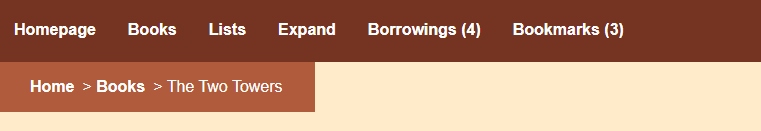
\includegraphics[scale=0.7]{images/application/navigation.png}
\caption{Navigation és Subnavigation}
\label{fig:navigation}
\end{figure}

\subsubsection{Layout komponens}

A \texttt{Layout} komponens biztosítja azt, hogy a \texttt{Navigation} komponens mindenhol szerepeljen. Ez úgy valósul meg, hogy az \texttt{App.js} fájlban a \texttt{Route}-okat tartalmazó \texttt{Switch} komponenst a \texttt{Layout} komponensen belül kell elhelyezni.

\subsection{Utility komponensek}

Az alábbi komponensek különböző kisegítő funkciókat biztosítanak más komponensek számára.

\subsubsection{LoadingSpinner komponens}

A \texttt{LoadingSpinner} komponens kerül felhasználásra amikor egy aszinkron kérésre kapott válaszra vár az adott komponens.

\subsubsection{Pagination komponens}

A \texttt{Pagination} komponens a \texttt{react-paginate} letölthető komponens segítségével valósul meg. A komponens létrehoz egy olyan felületet (\ref{fig:pagination}. ábra), ahol a felhasználó kiválaszthatja, hogy a találatok hanyadik szettjét szeretné megtekinteni. Például: Ha 80 találat van, és oldalanként 10 találatot kérünk, akkor 8 külön oldalon lesznek megjelenítve a találatok. A komponens jelzi, hogy jelenleg melyik oldalon vagyunk, és hogy hány elérhető oldal van. Egy oldalszámra kattintva megjelennek a kiválasztott oldalhoz tartozó találatok, az előre és hátra gombokra kattintva egy oldalt tudunk előre, vagy hátra lépni.

\begin{figure}[h]
\centering
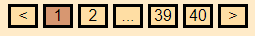
\includegraphics[scale=1]{images/application/pagination.png}
\caption{Navigation és Subnavigation}
\label{fig:pagination}
\end{figure}

A \texttt{Pagination} komponens más komponensekbe egyszerűen implementálható. Pro\-per\-ty-ként meg kell kapnia a jelenlegi oldalt, valamint egy függvényt, ami az oldal változását kezeli. Azt, hogy a találatok közül hanyadik oldalnak kell betöltődnie, az implementáló komponensek tartják számon. Amikor a komponensek lekérik az elemeket az adatbázisból, akkor mellékelniük kell hogy hanyadik oldalt kérik, hogy hogy hány darab találatot kérnek.

\subsubsection{YearSelector komponens}

A \texttt{YearSelector} komponens lehetőséget biztosít, hogy egy lenyíló menüből a felhasználó évszámot választhasson.

\Section{A backend megvalósítása}
% TODO: Mivel a backend aránylag egyszerű szerkezetű, ezért itt elég csak röviden bemutatni, hogy a routing hogy lett megoldva, és hogy szerkezetileg hogy épül fel az alkalmazás.
A backend \textit{NodeJS} és \textit{Express} segítségével valósul meg. A NodeJS egy nyílt forráskódú JavaScript környezet, amelynek segítségével szerver alkalmazásokat lehet készíteni. Az Express egy minimális és rugalmas NodeJS keretrendszer.

A szerver alkalmazás az Express keretrendszeren kívül más modulokat is felhasznál:
\begin{itemize}
    \item A \texttt{path} modul: Fájl és mappa elérési útvonalakkal való dolgozáshoz ad eszközöket.
    \item A \texttt{morgan} modul: Kérések naplózását végzi.
    \item A \texttt{cookie-parser} és \texttt{body-parser} modulok: Kérések törzseinek és sütijeinek elemzésére használatos.
\end{itemize}

Az útvonalak a \texttt{routes} mappában találhatóak, és az \texttt{index.js} fájlban kerülnek importálásra. A \texttt{config.js} fájlban kerül inicializálásra a Neo4j driver.

\Chapter{Adatkezelés Neo4j segítségével}

A mintaalkalmazás adatainak tárolása egy Neo4j által biztosított gráfadatbázisban történik. Ebben a fejezetben szó lesz arról, hogy milyen szolgáltatásokat biztosít a Neo4j a felhasználók számára, hogyan írhatjuk le az adatokat, hogy valósulnak meg a lekérdezések a Cypher lekérdező nyelv segítségével, hogy hogyan lehet kapcsolatot létesíteni az adatbázis és a mintaalkalmazás között, valamint arról, hogy a Neo4j milyen magasabb rendű hozzáférési módot biztosít.

\Section{Szoftveres eszközök}

A Neo4j számos szoftveres eszközt biztosít a gráfokkal való adatkezelés lebonyolításához. Ebben az alfejezetben ezen eszközök rövid bemutatására fog sor kerülni.

\subsection{Neo4j Graph Database}

A \textit{Neo4j Graph Database} a Neo4j Platform központi része. A Neo4j széles körben elterjedt, sikerrel alkalmazzák különféle tudományos, ipari és vállalati területeken, beleértve az élettudományokat, a közműveket, a pénzügyi szolgáltatásokat, a kiberbiztonságot és még sok mást \cite{neo4j-graph-database}.

A Neo4j Graph Database legfontosabb tulajdonságai közé tartozik
\begin{itemize}
      \item a gráfok automatikus, dinamikus átméretezése,
      \item a kiváló teljesítmény,
      \item a megbízható működés az üzemeltetés során,
      \item a felhő alapú rendszerekhez illeszkedő kialakítása, 
      \item a hatékony fejlesztés segítése.
\end{itemize}
A következő szakaszokban az eszközkészletének néhány eleme kerül említésre.

\subsection{Neo4j AuraDB}

A \textit{Neo4j AuraDB} egy felhőalapú gráfadatbázis szolgáltatás. 

\subsection{Neo4j Graph Data Science}

A \textit{Graph Data Science} segítségével ismeretekre lehet szert tenni az adatok összefüggéseiből és struktúráiból, jellemzően előrejelzésekhez . Olyan eszköztárat taralmaz, amely segít az adatkutatóknak megválaszolni kérdéseket és megmagyarázni az eredményeket grafikonokon ábrázolt adatok segítségével \cite{neo4j-graph-data-science}.

\subsection{Neo4j Developer Tools}

A Neo4j két fejlesztői felületet biztosít: egy letölthető és telepíthető asztali alkalmazást, és egy böngészőből futtatható alkalmazát.

\subsubsection{Neo4j Desktop}

A \textit{Neo4j Desktop} egy fejlesztői IDE (\textit{Integrated Development Environment}) vagy felügyeleti környezet \cite{neo4j-desktop}.
Tetszőleges számú lokális projektet és adatbázist lehet vele kezelni, valamint lehet vele csatlakozni távoli Neo4j szerverekhez is. 

A Neo4j Desktop által kezelt adatbázisok konfigurálhatók, frissíthetők és karbantarthatók a felhasználói felületen keresztül, parancssor nélkül. Lehetőséget biztosít Neo4j bővítmények telepítésére.

\subsubsection{Neo4j Browser}

A \textit{Neo4j Browser} egy böngészőből futtatható Neo4j interface lekérdezésekhez és adatok megjelenítéséhez. Cypher-szerkesztőt kínál szintaktikai kiemeléssel, kódkiegészítéssel és figyelmeztetésekkel, amelyek segítenek a Cypher lekérdezések írásakor \cite{neo4j-browser}.

\subsection{Neo4j Bloom}

A \textit{Neo4j Bloom} egy olyan eszköz, amely megjeleníthetővé teszi az adatokat egy gráfban, valamint lehetőséget biztosít lekérdezésekre lekérdező nyelv vagy programozási nyelv ismerete nélkül. A Bloom igénybe vehető a Neo4j Desktop és Neo4j Browser szolgáltatásokon keresztül \cite{neo4j-bloom1}, \cite{neo4j-bloom2}.

\subsection{Neo4j GraphQL Library}

A \textit{Neo4j GraphQL Library} egy rendkívül rugalmas, kevés kódolást igénylő (\textit{low code}), nyílt forráskódú JavaScript könyvtár, amely lehetővé teszi a gyors API-fejlesztést.

A Neo4j gráf adatbázissal a GraphQL Library egyszerűvé teszi az alkalmazások számára, hogy az alkalmazás adatokat natívan gráfként kezeljék a frontend-től egészen a tárolásig, elkerülve ezzel a séma duplikációt, és probléma mentes integrációt biztosítva a frontend és a backend között.

A könyvtár TypeScripten készült. A "Séma az első" (\textit{schema first}) paradigma lehetővé teszi a fejlesztők számára, hogy a szükséges alkalmazásadatokra összpontosítsanak, miközben a könyvtár gondoskodik az API felépítésének nehezéről  \cite{neo4j-graphql-library1}, \cite{neo4j-graphql-library2}.

\Section{Az adatok leírása}

A Neo4j egy típusos adatbázis, ami az alábbi típusokat tudja kezelni \cite{neo4j-values}:
\begin{itemize}
    \item Tulajdonság típusok: Integer, Float, String, Boolean, Point, Date, Time, LocalTime, DateTime, LocalDateTime, Duration,
    \item Strukturális típusok: Node, Relationship, Path,
    \item Összetett típusok: List, Map.
\end{itemize}

Neo4j-ben a csomópontok egyedeket reprezentálnak \cite{adatok-leirasa}. A csomópontokhoz tartozhatnak úgynevezett címkék, amik leírják, hogy milyen típusú az adott csomópont. Egy csomóponthoz tartozhat nulla, egy, vagy több címke. Például a mintaalkalmazásban található könyvek \textit{Book} címkével ellátott csomópontokként kerülnek ábrázolásra az adatbázisban.

Az élek két csomópont közötti kapcsolatot reprezentálnak. Egy kapcsolatnak mindig van iránya és típusa. Például a mintaalkalmazásban egy könyv felhasználó általi értékelését követően a felhasználó és a könyv csomópontok között létrejön egy \textit{Rated} kapcsolat.

Csomópontok és kapcsolatok rendelkezhetnek tulajdonságokkal, amik kulcs-érték párok. Például egy könyvhöz tartozhat szerző tulajdonság.

\Section{Lekérdezések}

Neo4j-ben a lekérdezések a \textit{Cypher Query Language} segítségével valósulnak meg. A Cypher egy SQL által inspirált lekérdező nyelv, ezért ebben az alfejezetben egyaránt bemutatásra kerül, hogy bizonyos műveletek hogyan valósíthatók meg Cypherrel és SQL-el \cite{cypher}, \cite{sql}.

\subsection{Kiválasztás}

Cypher-ben az adatok kiválasztása a \texttt{MATCH} paranccsal történik, amiket a kiválasztást követően a \texttt{RETURN} paranccsal lehet megkapni. A következő parancs lekérdezi az adatbázisban található összes könyvet.
\begin{java}[columns=fullflexible]
MATCH (n:Book) RETURN n
\end{java}
Az alábbi parancs pedig a Stephen King által írt könyveket fogja lekérdezni.
\begin{java}[columns=fullflexible]
MATCH (n:Book{author: "Stephen King"}) RETURN n
\end{java}
Az \texttt{OPTIONAL MATCH} parancs hasonlóan működik mint a \texttt{MATCH}, annyi eltéréssel, hogy ha nincs találat, akkor az \texttt{OPTIONAL MATCH} null értéket fog használni a minta hiányzó részeinél. A következő parancs az adatbázisban található könyveket fogja visszaadni, és ha van hozzájuk értékelés, akkor azoknak az átlagát is. Amennyiben nincs, akkor az átlag helyén null érték fog szerepelni.
\begin{java}[columns=fullflexible]
MATCH (b:Book) 
OPTIONAL MATCH (a)-[r:Rated]->(b) 
RETURN b.title, avg(r.rating)
\end{java}
SQL-ben a \texttt{MATCH} megfelelője a \texttt{SELECT} paranccsal, míg az \texttt{OPTIONAL MATCH} megfelelője az \texttt{OUTER JOIN}:
\begin{java}[columns=fullflexible]
SELECT * FROM Books;
SELECT * FROM Books WHERE Author='Stephen King';
SELECT Books.Title, AVG(Rated.Rating) FROM Books 
FULL OUTER JOIN Rated USING(BookID) GROUP BY Books.Title;
\end{java}

\subsection{Korlátozás}
A \texttt{WHERE} paranccsal korlátozásokat lehet hozzárendelni a \texttt{MATCH} és \texttt{OPTIONAL MATCH} parancsokhoz. A \texttt{WHERE} paranccsal lehet vizsgálni például egy csomópont vagy kapcsolat ID-jét, címkéjét és tulajdonságait, számok közötti egyenlőséget illetve egyenlőtlenséget, szöveges egyezést. Az alábbi parancs a 24-es ID-vel rendelkező könyv adatait fogja visszaadni.
\begin{java}[columns=fullflexible]
MATCH (b:Book) 
WHERE ID(b)=24
RETURN b
\end{java}

\subsection{Létrehozás}
Cypher-rel az adatbázisban csomópontot és kapcsolatot a \texttt{CREATE} paranccsal lehet létrehozni. A következő lekérdezés létrehoz egy könyvet az adatbázisban a megadott tulajdonságokkal. A parancsban az \textit{n} egy változó, a \textit{Book} egy címke, míg az \textit{author} és a \textit{title} tulajdonságok. 
\begin{java}[columns=fullflexible]
CREATE(n:Book{
  author:"J. R. R. Tolkien",
  title:"The Two Towers"
})
\end{java}
Az alábbi parancs egy kapcsolatot fog létrehozni a megadott felhasználó és megadott könyv között a megadott névvel.
\begin{java}[columns=fullflexible]
MATCH (a:User), (b:Book) 
WHERE ID(a)=112 AND ID(b)=23
CREATE (a)-[r:Bookmarked]->(b) 
\end{java}
SQL-ben adat rögzítéséhez először egy táblát kell létrehozni, majd ezt követően lehet azt feltölteni adatokkal.
\begin{java}[columns=fullflexible]
CREATE TABLE Books(
  BookID INT PRIMARY KEY NOT NULL,
  Author VARCHAR(30),
  Title VARCHAR(30)
);
INSERT INTO Books
VALUES (1, 'J. R. R. Tolkien', 'The Two Towers');
\end{java}
A Cypher-beli kapcsolatot SQL-ben egyedi és idegen kulcsokkal lehet megvalósítani. Az alábbi példában kapcsolótábla kerül alkalmazásra:
\begin{java}[columns=fullflexible]
CREATE TABLE Bookmarked(
  UserID INT, 
  FOREIGN KEY(UserID) REFERENCES Users(UserID),
  BookID INT, 
  FOREIGN KEY(BookID) REFERENCES Books(BookID)
);
INSERT INTO Bookmarked VALUES (112, 23);
\end{java}

\subsection{Törlés}
Csomópontok és kapcsolatok törlésére a \textit{DELETE} paranccsal van lehetőségünk. Az alábbi lekérdezés törölni fogja a megadott csomópontot, amennyiben az nem rendelkezik kapcsolatokkal.
\begin{java}[columns=fullflexible]
MATCH (n:Book) 
WHERE ID(n)=24 
DELETE n
\end{java}
Amennyiben olyan csomópontot szeretnénk törölni, amihez tartozik kapcsolat, akkor a \texttt{DETACH DELETE} parancsot kell használni.
\begin{java}[columns=fullflexible]
MATCH (n:Book) 
WHERE ID(n)=24
DETACH DELETE n
\end{java}
A következő parancs megszünteti a \texttt{Bookmarked} kapcsolatot a megadott felhasználó és a megadott könyv között.
\begin{java}[columns=fullflexible]
MATCH (a:User)-[r:Bookmarked]->(b:Book) 
WHERE ID(a)=12 AND ID(b)=14
DELETE r
\end{java}
SQL-ben a törlés a \texttt{DELETE} paranccsal történik.
\begin{java}[columns=fullflexible]
DELETE FROM Books 
WHERE BookID = 24;
\end{java}

\subsection{Rendezés}
Cypher-ben az \texttt{ORDER BY} paranccsal lehet a találatokat rendezni. Az alábbi parancs a könyv darabszáma alapján csökkenő sorrendben fogja visszaadni a találatokat.
\begin{java}[columns=fullflexible]
MATCH (n:Book) 
RETURN n.stock 
ORDER BY n.stock DESC
\end{java}
SQL-ben szintén az \texttt{ORDER BY} paranccsal történik a rendezés.
\begin{java}[columns=fullflexible]
SELECT * 
FROM Books 
ORDER BY Stock DESC;
\end{java}

\subsection{Kihagyás}
Cypher-ben a \texttt{SKIP} paranccsal át lehet ugrani a megadott mennyiségű első találatot. A következő parancs a könyv darabszáma alapján fogja rendezni a találatokat csökkenő sorrendben, majd ezek közül kihagy 1-et, és visszaadja a többit.
\begin{java}[columns=fullflexible]
MATCH (n:Book) 
RETURN n.stock 
ORDER BY n.stock DESC
SKIP 1
\end{java}
SQL-ben elem kihagyására az \texttt{OFFSET} paranccsal van lehetőség.
\begin{java}[columns=fullflexible]
SELECT * 
FROM Books 
ORDER BY Stock DESC
OFFSET 1;
\end{java}

\subsection{Limitálás}
Cypher-ben a \texttt{LIMIT} paranccsal meg lehet adni, hogy hány találatot szeretnénk megkapni. Az alábbi parancs a könyv darabszáma alapján fogja rendezni a találatokat csökkenő sorrendbe, de csak az első két találatot adja vissza.
\begin{java}[columns=fullflexible]
MATCH (n:Book) 
RETURN n.stock 
ORDER BY n.stock DESC
LIMIT 2
\end{java}
SQL-ben hasonlóképpen használható a \texttt{LIMIT} parancs.
\begin{java}[columns=fullflexible]
SELECT *
FROM Books 
ORDER BY Stock DESC
LIMIT 2;
\end{java}
Alternatívaként használható az alábbi, \texttt{FETCH} paranccsal megadott lekérdezés is.
\begin{java}[columns=fullflexible]
SELECT *
FROM Books 
ORDER BY Stock DESC;
FETCH FIRST 2 ROWS ONLY;
\end{java}

A \texttt{SKIP} és \texttt{LIMIT}, illetve \texttt{OFFSET} és \texttt{FETCH} parancsokat gyakran együtt használják a webalkalmazásokban a lapozás (\textit{pagination}) megvalósításához.

\subsection{Frissítés}
Cypher-ben a \texttt{SET} paranccsal lehet tulajdonságokat és címkéket létrehozni, értéküket megváltoztatni, illetve törölni. Az alábbi parancs a megadott ID-jű könyv kategóriáját \textit{Fantasy}-ra fogja beállítani.
\begin{java}[columns=fullflexible]
MATCH (n:Book) 
WHERE ID(n)=24
SET n.category="Fantasy"
\end{java}
SQL-ben ez az \texttt{UPDATE} paranccsal történik.
\begin{java}[columns=fullflexible]
UPDATE Books
SET Category = 'Fantasy'
WHERE BookID = 24;
\end{java}

\Section{Kapcsolódás az adatbázishoz}

A Neo4j-hez igénybe vehető számos hivatalos meghajtóprogram (\textit{driver}), amik egyszerűsítik egy alkalmazás és az adatbázis összekapcsolását. Az alábbi programozási nyelvekhez érhető el hivatalos kiadás:
\begin{itemize}
    \item .NET,
    \item Go,
    \item Java,
    \item JavaScript,
    \item Python.
\end{itemize}
JavaScript esetében a kapcsolódás az alábbi módon történik:
\begin{itemize}
\item Neo4j driver telepítése:
\begin{java}
npm install neo4j-driver
\end{java}
\item Neo4j driver importálása: 
\begin{java}
const neo4j = require("neo4j-driver");
\end{java}
\item Neo4j driver inicializálása:
\begin{java}
const driver = neo4j.driver(
  uri,
  neo4j.auth.basic(user, password)
);
\end{java}
\end{itemize}

\Section{Lekérdezések kiadása}
A mintaalkalmazásban a lekérdezések kiadására a \textit{Neo4j Driver}-ben található \textit{Session API} kerül felhasználásra \cite{neo4j-session-api}. Ahhoz, hogy elkezdhessük használni a \textit{Session API}-t, először is deklarálnunk kell a \texttt{session} objektumot:
\begin{java}
const session = driver.session()
\end{java}

Ezt követően a \texttt{run} függvény segítségével futtathatjuk a lekérdezéseket az alábbi módon:
\begin{java}
session.run(query, queryParams);
\end{java}
 
A \texttt{query} az maga a lekérdezés sztring formátumban, a \texttt{queryParams} pedig egy opcionális objektum, ami tartalmazza a lekérdezéshez tartozó paramétereket. Például, az alábbi példában azt a felhasználót keressük, akinek az ID-je megegyezik a \texttt{userId} változóban szereplő értékkel. A lekérdezésben a \texttt{\$userIdParam} jelzi, hogy oda egy paramétert vár.
\begin{java}[columns=fullflexible]
const query = `
  MATCH(n:User) 
  WHERE ID(n)=$userIdParam 
  RETURN n`;
  
const queryParams = {
  userIdParam: userId
};
\end{java}

A \texttt{run} függvény futtatása után a \texttt{then} függvénnyel lehet a kapott választ feldolgozni. Az alábbi példában ez kerül kiírásra:
\begin{java}
session.run(query, queryParams)
  .then(function (result) {
    console.log(result)
  }
);
\end{java}

\Section{Magasabb szintű hozzáférési módok}
Magasabb hozzáférési módként a Neo4j objektum gráf leképzést (\textit{OGM, Object Graph Mapper}) ajánl. Az OGM a gráf csomópontjait és kapcsolatait képezi le objektumokra és hivatkozásokra az alábbi módon:
\begin{itemize}
    \item Az objektumpéldányokat csomópontokra képzi.
    \item Az objektumhivatkozásokat kapcsolatokra képzi.
    \item A JVM primitíveket csomópont- vagy kapcsolattulajdonságokra képzi.
\end{itemize}

Az OGM elvonatkoztatja az adatbázist, és kényelmes módot biztosít a tartománymodell grafikonon való megtartására és lekérdezésére alacsony szintű illesztőprogramok használata nélkül. Rugalmasságot biztosít a fejlesztő számára egyéni lekérdezésekhez, ha a Neo4j-OGM által generált lekérdezések nem elegendőek.

A Neo4j a \textit{Neo4j-OGM} könyvtárat biztosítja az OGM-hez. Ez egy Java könyvtár, amely a Neo4j használatával képes megőrizni a tartományobjektumokat. Cypher utasításokat használ a műveletek kezelésére.

\Chapter{Optimalizálás és adatbázis menedzsment}

Ebben a fejezetben webalkalmazások és a Neo4j adatbázis jogosultságkezeléséről és gyosrítótárazásáról lesz szó, valamint a Neo4j adatbázis konfigurálási és biztonsági mentés lehetőségei kerülnek bemutatásra.

\Section{Jogosultságkezelés}

Webalkalmazások esetén szükséges lehet, hogy bizonyos felhasználó csoportok különböző szinten tudjanak hozzáférni az alkalmazáshoz. Például a mintaalkalmazásban a felhasználók 3 csoportra vannak bontva: nem bejelentkezett felhasználó, bejelentkezett  felhasználó, és adminisztrátor jogosultságú felhasználó. Egy nem bejelentkezett felhasználó az alkalmazás csak egy részével tud interaktálni, egy bejelentkezett felhasználó az admin funkciók kivételével minden funkciót igénybe tud venni, míg az admin jogosultsággal rendelkező felhasználó az alkalmazás minden funkcióját ki tudja használni.

Neo4j-ben lehetőség van úgynevezett szerep alapú hozzáférés-szabályozásra \cite{neo4j-privileges}. Ez a szolgáltatás csak az \textit{Enterprise Edition}-ben érhető el. Hozzáférést a \texttt{GRANT} és a \texttt{DENY} parancsokkal lehet szabályozni. A megadott illetve a megtagadott hozzáférést a \texttt{REVOKE} paranccsal lehet semmissé tenni. 

\Section{Gyorsítótárazás}

A gyorsítótárazás (\textit{caching}) segítségével adatokat lehet tárolni a helyi merevlemezen annak érdekében, hogy a lekérdezésekre gyorsabban tudjon válaszolni a webalkalmazás \cite{cache}. A gyorsítótárazás kis méretű statikus adatok kezelésére szolgál, például képek, CSS és JavaScript fájlok. Gyorsítótárazás esetén fontos, hogy a tárolt adatok ne váljanak elavulttá. Az elavultság megelőzésének érdekében minden gyorsítótárazási mechanizmusnak tudnia kell szabályozni a tartalom frissítésének időpontját. Például egy weboldal megnyitásakor a böngésző ellenőrzi, hogy a gyorsítótárban lévő adatok frissek-e. Ha igen, akkor betölti azokat, ha nem, akkor letölti az adatok friss verzióját (egyúttal frissíti a gyorsítótárat).

Neo4j-ben lehetőség van az úgynevezett \textit{page cache} használatára. Ez a Neo4j által használt adatok gyorsítótárazására szolgál. Gráf adatokat és indexeket tárol vele a memóriában \cite{neo4j-page-cache}.

\Section{Konfigurálási lehetőségek}

A Neo4j adatbázis konfigurációs beállításai a \texttt{neo4j.conf} fájlban találhatóak. A legtöbb beállítás a Neo4j-re vonatkozik, de bizonyos beállítások a Java futtatókörnyezethez kapcsolódik, ugyanis a Neo4j ezen fut.

Néhány érdekesebb konfigurálási lehetőség \cite{neo4j-config-settings}:
\begin{itemize}
    \item \texttt{dbms.backup.enabled} - Online biztonsági mentések készítését szabályozza.
    \item \texttt{dbms.db.timezone} - Az adatbázis időzónáját szabályozza.
    \item \texttt{dbms.default\_database} - Azt szabályozza, hogy melyik legyen az alapértelmezett adatbázis.
    \item \texttt{dbms.read\_only} - Ha be van kapcsolva, akkor csak olvasási operációk futtathatók.
\end{itemize}

\Section{Biztonsági mentések}

A Neo4j többfajta lehetőséget is biztosít biztonsági mentések létrehozására \cite{neo4j-backup}.

\begin{itemize}
    \item \textit{Backup és Restore}: Online biztonsági mentések létrehozására és azokat felhasználva adatbázis visszaállítás végrehajtására használható módszer. (Csak az \textit{Enterprise Edition}-el használható.)
    \item \textit{Copy}: Offline adatbázisok esetében adatbázis-ellentmondások megszüntetésére, fel nem használt tárhely felszabadítására, valamint régebbi verzióról új verzióra váltásra lehet használni. (Szintén csak az \textit{Enterprise Edition}-el használható.)
    \item \textit{Dump és Load}: Offline biztonsági mentések létrehozására és azokat felhasználva adatbázis visszaállítás végrehajtására használható módszer. A mentés létrehozásakor létrejön egy \texttt{.dump} kiterjesztésű fájl, amit ezután fel lehet használni az adatbázis visszaállítására.
\end{itemize}
\Chapter{Összefoglalás}

% TODO: Össze kell foglalni a tapasztalatokat, hogy milyen szempontból volt előnyös/hátrányos a gráfadatbázis, azokon belül is a Neo4j használata.

% Ezt is bőven elég csak akkor megírni, hogy ha már a dolgozat többi része kész van.

A dolgozatban egy könyvtári alkalmazás példáján keresztül került bemutatásra az, hogy egy webalkalmazás elkészítése során az adatok kezelése hogyan oldható meg a Neo4j gráfadatbázis segítségével.
A példa megválasztásánál szempontként szerepelt, hogy minden gyakori lekérdezés típus bemutatható legyen a segítségével, így általános képet adva arról, hogy azok hogyan szervezhetők gráfba, és milyen eszközöket adottak a lekérdezésekhez és a fejlesztéshez.

A Neo4j féle gráfadatbázissal egyszerű volt megoldani a mintaalkalmazás adatainak kezelését. A fejlesztők által készített dokumentáció nagyon részletes és sok példát tartalmaz, ezért könnyű volt elsajátítani az alapokat. Mivel a Neo4j az egyik legelterjedtebb gráfadatbázis, sok más forrásból is lehetett tanulni. Megjegyzendő, hogy mivel nem annyira elterjedt, mint például a relációs adatbáziskezelő rendszerek, ezért voltak esetek, ahol nehezen lehetett információt találni egy-egy problémával kapcsolatban. 

A Neo4j Aura segítségével egyszerű volt az adatbázis futtatása. Az ingyenes verzió 50 ezer csomópont, és 175 ezer kapcsolat létrehozását támogatja, ami bőven elég volt a minta alkalmazás számára. Hátránya, hogy pár nap inaktivitás után az adatbázist automatikusan szüneteltetik, amit ezt követően manuálisan kell visszakapcsolni.

A Neo4j által készített JavaScript driver és a Session API segítségével sikerült megoldani a mintaalkalmazás és az adatbázis összekapcsolását. Lekérdezések esetében a paraméterek megadása nem minden esetben volt kézenfekvő.

A Neo4j grafikus felületével kellemes volt dolgozni, az adatbázisba felvitt adatok látványosan megjeleníthetők. Sokszor már csak ránézésből is meg lehetett állapítani, hogy egy lekérdezés helyesen működik-e.

Összeségében egyszerűen és hatékonyan fel tudtam építeni a minta alkalmazás adatait tároló gráfadatbázist a Neo4j által nyújtott eszközökkel.


\clearpage

\addcontentsline{toc}{chapter}{Irodalomjegyzék}
\bibliographystyle{unsrt}
\bibliography{dolgozat.bib}

\newpage

\pagestyle{empty}

\noindent \textbf{\Large CD Használati útmutató}

\vskip 1cm

\noindent A CD tartalmazza az alábbiakat:
\begin{itemize}
    \item a szakdolgozat PDF formátumban,
    \item a szakdolgozat \LaTeX\ forráskódja,
    \item a mintaalkalmazás forráskódja,
    \item tesztadatbázis,
    \item API dokumentáció,
    \item CD Használati útmutató.
\end{itemize}

\bigskip

A CD-n található mintaalkalmazás futtatásához a klienshez és a backendhez is telepíteni kell a szükséges csomagokat. Az alkalmazás gyökérkönyvtárából kiindulva:
\begin{itemize}
    \item Szerver: \texttt{npm install}
    \item Kliens: \texttt{cd client}, ezt követően \texttt{npm install}
\end{itemize}

Ez után külön terminálokon futtatni kell mindkettőt. Az alkalmazás gyökérkönyvtárából kiindulva:
\begin{itemize}
    \item Szerver: \texttt{npm start}
    \item Kliens: \texttt{cd client}, ezt követően \texttt{npm start}
\end{itemize}

A tesztadatbázis a \texttt{tesztadatbazis.dump} fájlban található. Ezt a fájlt egy Neo4j gráfadatbázisba kell importálni. Neo4j Aura esetében az adatbázis létrehozásakor kapott felhasználónevet, jelszót és URI-t az alkalamzás \texttt{server.js} fájlban kell megadni.

\bigskip

A könyvek borítóképei a \textit{FireBase Storage}-be kerülnek feltöltésre.  Mivel a borítóképek elérési útvonala függ a projekt nevétől, a tesztadatbázisban található könyvek borítóképei nem fognak megjelenni, ha a \textit{FireBase Storage}, amin a képek vannak, nem elérhető. Amennyiben az eredeti \textit{FireBase Storage} még aktív, akkor nincs további teendő. Ha inaktív, akkor ahhoz, hogy a borítóképek működjenek, egy új \textit{FireBase Storage}-t kell létrehozni, majd összekapcsolni vele az alkalmazást. Először létre kell hozni egy új \textit{FireBase} projektet, majd telepíteni kell a \texttt{firebase} csomagot. Ezt követően be kell jelentkezni, inicializálni a projektet, majd beállítani a \texttt{storage}-t. Az \texttt{AdminNewBook.js} fájlban kell átírni a \texttt{projectId}-t az aktuális projektnek megfelelően. Ezt követően az új könyvek már az új \textit{FireBase Storage}-be kerülnek feltöltésre. A régi könyvek borítóképei megtalálhatók a tesztadatbázis mappájában. Ahhoz, hogy ezek megjelenjenek, fel kell őket tölteni manuálisan, majd a könyvek borítóképeinek a linkjét át kell írni az adatbázisban az újakra.

\end{document}
